\documentclass[10pt,a4paper]{article}
\usepackage[UTF8,fontset = windows]{ctex}
\setCJKmainfont[BoldFont=黑体,ItalicFont=楷体]{华文中宋}
\usepackage{amssymb,amsmath,amsfonts,amsthm,mathrsfs,dsfont,graphicx}
\usepackage{ifthen,indentfirst,enumerate,color,titletoc}
\usepackage{tikz}
\usepackage{multicol}
\usepackage{makecell}
\usepackage{longtable}
\usepackage{diagbox}
\usetikzlibrary{arrows,calc,intersections,patterns,decorations.pathreplacing,3d,angles,quotes,positioning}
\usepackage[bf,small,indentafter,pagestyles]{titlesec}
\usepackage[top=1in, bottom=1in,left=0.8in,right=0.8in]{geometry}
\renewcommand{\baselinestretch}{1.65}
\newtheorem{defi}{定义~}
\newtheorem{eg}{例~}
\newtheorem{ex}{~}
\newtheorem{rem}{注~}
\newtheorem{thm}{定理~}
\newtheorem{coro}{推论~}
\newtheorem{axiom}{公理~}
\newtheorem{prop}{性质~}
\newcommand{\blank}[1]{\underline{\hbox to #1pt{}}}
\newcommand{\bracket}[1]{(\hbox to #1pt{})}
\newcommand{\onech}[4]{\par\begin{tabular}{p{.9\textwidth}}
A.~#1\\
B.~#2\\
C.~#3\\
D.~#4
\end{tabular}}
\newcommand{\twoch}[4]{\par\begin{tabular}{p{.46\textwidth}p{.46\textwidth}}
A.~#1& B.~#2\\
C.~#3& D.~#4
\end{tabular}}
\newcommand{\vartwoch}[4]{\par\begin{tabular}{p{.46\textwidth}p{.46\textwidth}}
(1)~#1& (2)~#2\\
(3)~#3& (4)~#4
\end{tabular}}
\newcommand{\fourch}[4]{\par\begin{tabular}{p{.23\textwidth}p{.23\textwidth}p{.23\textwidth}p{.23\textwidth}}
A.~#1 &B.~#2& C.~#3& D.~#4
\end{tabular}}
\newcommand{\varfourch}[4]{\par\begin{tabular}{p{.23\textwidth}p{.23\textwidth}p{.23\textwidth}p{.23\textwidth}}
(1)~#1 &(2)~#2& (3)~#3& (4)~#4
\end{tabular}}
\begin{document}

\begin{enumerate}[1.]

%zmj1
\item 已知集合$A=\{y| y=\sin x , \ x\in \mathbf{R}\}$, 集合$B=\{y| y=\sqrt {x} , \ x\in \mathbf{R}\}$, 则$A\cap B=$\blank{50}.
\item 已知$1+\mathrm{i}$是实系数一元二次方程$x^2+ax+b=0$的根($i$为虚数单位), 则$2a+b=$\blank{50}.
\item 已知关于$x,y$的二元一次方程组的增广矩阵为$\begin{pmatrix}
   2 & 1 & 5  \\ 1 & -2 & 0  \end{pmatrix}$, 则$xy=$\blank{50}.	
\item 已知球的主视图的面积为$\dfrac{\pi}4$, 则该球的体积为\blank{50}.
\item 在平面直角坐标系$xOy$中, 直线$l$的参数方程为$\begin{cases} x=t-1, \\ y=t, \end{cases}$($t$为参数) 圆$O$的参数方程为$\begin{cases} x=\cos \theta,  \\ y=\sin \theta,  \end{cases}$($\theta$为参数) 则直线$l$与圆$O$的位置关系是\blank{50}.
\item 已知实数$x$、$y$满足条件$\begin{cases} x-y\ge 0, \\ y\ge 0, \\ x+y\le 1, \end{cases}$ 则目标函数$z=2x-y$的最大值为\blank{50}.
\item 方程$(\log_3x)^2+\log_93x=2$的解集为\blank{50}.
\item 某校高一、高二、高三共有$200$名学生, 为调查他们的体育锻炼情况, 通过分层抽样获得了20名学生一周的锻炼时间, 数据如下表(单位: 小时):
\begin{center}
\begin{tabular}{|c|c|c|c|c|c|c|c|c|}
\hline
高一 & $6$ & $6.5$ & $7$ & $7.5$ & $8$ & $$ & $$ & $$ \\ \hline
高二 & $6$ & $7$ & $8$ & $9$ & $10$ & $11$ & $12$ & $$ \\ \hline
高三 & $3$ & $4.5$ & $6$ & $7.5$ & $9$ & $10.5$ & $12$ & $13.5$ \\ \hline
\end{tabular}
\end{center}
则根据上述样本数据估计该校学生一周的锻炼时间不小于$7$小时的人数为\blank{50}.
\item 从$m$($m\in \mathbf{N}^*$, $m\ge 4$)个男生、$6$个女生中任选$2$个人当发言人, 假设事件$A$表示选出的$2$个人性别相同, 事件$B$表示选出的$2$个人性别不同. 如果$A$的概率和$B$的概率相等, 则$m=$\blank{50}.
\item 将函数$f(x)=2\sin 2x$的图像向左平移$\dfrac{\pi }6$个单位, 再向下平移$1$个单位, 得到函数的$y=g(x)$图像. 若$y=g(x)$在$[0,b]$($b>0$)上至少含有$2021$个零点, 则$b$的最小值为\blank{50}.
\item 如图, 在$\triangle ABC$中, $\angle BAC=\dfrac{\pi}3$, $D$为$AB$中点, $P$为$CD$上一点, 且满足$\overrightarrow{AP}=t\overrightarrow{AC}+\dfrac 13\overrightarrow{AB}$, 若$\triangle ABC$的面积为$\dfrac{3\sqrt 3}2$, 则$|\overrightarrow{AP}|$的最小值为\blank{50}.
\begin{center}
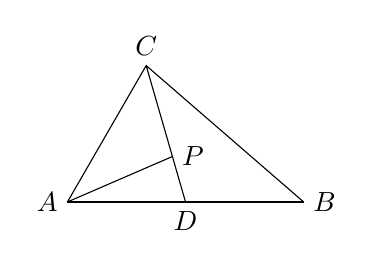
\begin{tikzpicture}[>=latex]
\draw (0,0) node [left] {$A$} coordinate (A) -- (1.5,0) node [below] {$D$} coordinate (D) -- (3,0) node [right] {$B$} coordinate (B);
\draw (60:2) node [above] {$C$} coordinate (C);
\draw ($(C)!{2/3}!(D)$) node [right] {$P$} coordinate (P);
\draw (A) -- (C) -- (B) (A) -- (P) (C) -- (D);
\end{tikzpicture}
\end{center}
\item 已知数列$\{a_n\}$, $\{b_n\}$满足$a_1=b_1=1$, 对任何正整数$n$均有$a_{n+1}=a_n+b_n+\sqrt {a_n^2+b_n^2}$, $b_{n+1}=a_n+b_n-\sqrt {a_n^2+b_n^2}$, 设$c_n=3^n(\dfrac 1{a_n}+\dfrac 1{b_n})$, 则数列$\{c_n\}$的前$2020$项之和为\blank{50}.
\item 已知实数$a\ne 0$, 则``$a<1$''是``$\dfrac 1a>1$''的\blank{50}\bracket{20}
\twoch{充分非必要条件}{必要非充分条件}{充要条件}{既非充分又非必要条件}
\item 如图, 正方体$A_1B_1C_1D_1-ABCD$中, $E$、$F$分别为棱$A_1A$、$BC$上的点, 在平面$ADD_1A_1$内且与平面$DEF$平行的直线\bracket{20}.
\begin{center}
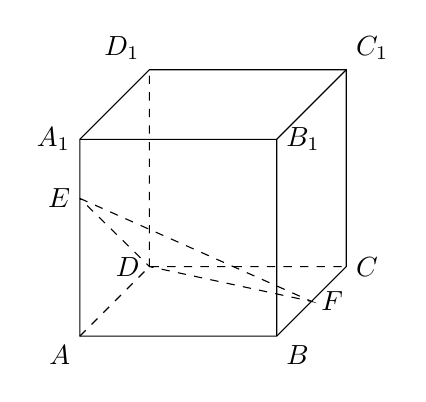
\begin{tikzpicture}[>=latex]
\draw (0,0) node [below left] {$A$} coordinate (A) --++ (2.5,0) node [below right] {$B$} coordinate (B) --++ (45:{2.5/2}) node [right] {$C$} coordinate (C)
--++ (0,2.5) node [above right] {$C_1$} coordinate (C1)
--++ (-2.5,0) node [above left] {$D_1$} coordinate (D1) --++ (225:{2.5/2}) node [left] {$A_1$} coordinate (A1) -- cycle;
\draw (A) ++ (2.5,2.5) node [right] {$B_1$} coordinate (B1) -- (B) (B1) --++ (45:{2.5/2}) (B1) --++ (-2.5,0);
\draw [dashed] (A) --++ (45:{2.5/2}) node [left] {$D$} coordinate (D) --++ (2.5,0) (D) --++ (0,2.5);
\draw ($(B)!0.5!(C)$) node [right] {$F$} coordinate (F);
\draw ($(A)!0.7!(A1)$) node [left] {$E$} coordinate (E);
\draw [dashed] (E) -- (F) -- (D) -- cycle;
\end{tikzpicture}
\end{center}
\fourch{有一条}{有二条}{有无数条}{不存在}
\item 已知函数$f(x)$($x\in D$), 若对任意的$x\in D$, 都存在$t\in D$, 使$f(t)=-f(x)$成立, 称$f(x)$是``拟奇函数''. 下列函数是``拟奇函数''的个数是\bracket{20}.\\
\textcircled{1} $f(x)=x^2$;  \textcircled{2} $f(x)=\ln x$;  \textcircled{3} $f(x)=x+\dfrac 1x$;  \textcircled{4} $f(x)=\cos x$
\fourch{$1$个}{$2$个}{$3$个}{$4$个}
\item 设集合$S=\{1,2,3,\cdots,2020\}$, 设集合$A$是集合$S$的非空子集, $A$中的最大元素和最小元素之差称为集合$A$的直径. 那么集合$S$所有直径为$71$的子集的元素个数之和为\bracket{20}.
\fourch{$71\cdot 1949$}{$2^{70}\cdot 1949$}{$2^{70}\cdot 37\cdot 1949$}{$2^{70}\cdot 72\cdot 1949$}
\item 如图所示的几何体是圆柱的一部分, 它是由边长为$2$的正方形$ABCD$(及其内部)以$AB$边所在直线为旋转轴顺时针旋转$120^{\circ}$得到的.
\begin{center}
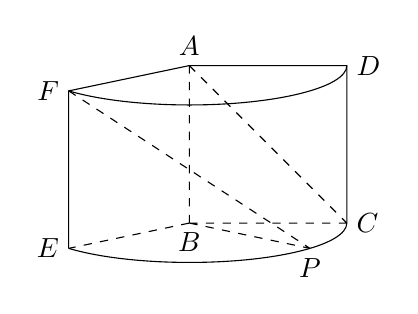
\begin{tikzpicture}[>=latex]
\draw (0,0) node [below] {$B$} coordinate (B);
\draw (2,0) node [right] {$C$} coordinate (C);
\draw (2,2) node [right] {$D$} coordinate (D);
\draw (0,2) node [above] {$A$} coordinate (A);
\draw ({2*cos(-140)},{0.5*sin(-140)}) node [left] {$E$} coordinate (E);
\draw (E) ++ (0,2) node [left] {$F$} coordinate (F);
\draw ({2*cos(-40)},{0.5*sin(-40)}) node [below] {$P$} coordinate (P);
\draw (E) -- (F) -- (A) -- (D) -- (C) arc (0:-140:2 and 0.5);
\draw (D) arc (0:-140:2 and 0.5);
\draw [dashed] (B) -- (A) (B) -- (E) (B) -- (C) (A) -- (C) (F) -- (P) (B) -- (P);
\end{tikzpicture}
\end{center}
(1) 求此几何体的体积;\\
(2) 设$P$是弧$EC$上的一点, 且$BP\perp BE$, 求异面直线$FP$与$CA$所成角的大小. (结果用反三角函数值表示)
\item 已知锐角$\alpha$、$\beta$的顶点与坐标原点重合, 始边与$x$轴正方向重合, 终边与单位圆分别交于$P$、$Q$两点, 若$P$、$Q$两点的横坐标分别为$\dfrac{3\sqrt {10}}{10}$、$\dfrac{2\sqrt 5}5$.\\
(1) 求$\cos (\alpha +\beta)$的大小;\\
(2) 在$\triangle ABC$中, $a,b,c$为三个内角$A,B,C$对应的边长, 若已知角$C=\alpha +\beta$, $\tan A=\dfrac 34$, 且$a^2=\lambda bc+c^2$, 求$\lambda$的值.
\item 疫情后, 为了支持企业复工复产, 某地政府决定向当地企业发放补助款, 其中对纳税额在$3$万元至$6$万元(包括$3$万元和$6$万元)的小微企业做统一方案. 方案要求同时具备下列两个条件: \textcircled{1} 补助款$f(x)$(万元)随企业原纳税额$x$(万元)的增加而增加; \textcircled{2} 补助款不低于原纳税额$x$(万元)的$50\%$. 经测算政府决定采用函数模型$f(x)=\dfrac x4-\dfrac bx+4$(其中$b$为参数)作为补助款发放方案.\\
(1) 判断使用参数$b=12$是否满足条件, 并说明理由;\\
(2) 求同时满足条件\textcircled{1}、\textcircled{2}的参数$b$的取值范围.
\item 在平面直角坐标系$xOy$中, $F_1$, $F_2$分别是椭圆$\Gamma :\dfrac{x^2}{a^2}+y^2=1$($a>0$)的左、右焦点, 直线$l$与椭圆交于不同的两点$A$, $B$, 且$|AF_1|+|AF_2|=2\sqrt 2$.\\
(1) 求椭圆$\Gamma$的方程;\\
(2) 已知直线$l$经过椭圆的右焦点$F_2$, $P,Q$是椭圆上两点, 四边形$ABPQ$是菱形, 求直线$l$的方程;\\
(3) 已知直线$l$不经过椭圆的右焦点$F_2$, 直线$AF_2$, $l$, $BF_2$的斜率依次成等差数列, 求直线$l$在$y$轴上截距的取值范围.
\item 若数列$\{a_n\}$对任意连续三项$a_i,a_{i+1},a_{i+2}$, 均有$(a_i-a_{i+2})(a_{i+2}-a_{i+1})>0$, 则称该数列为``跳跃数列''.\\
(1) 判断下列两个数列是否是跳跃数列:\\
\textcircled{1} 等差数列: $1,2,3,4,5,\cdots$; \textcircled{2} 等比数列: $1,-\dfrac 12,\dfrac 14,-\dfrac 18,\dfrac 1{16},\cdots$;\\
(2) 若数列$\{a_n\}$满足对任何正整数$n$, 均有$a_{n+1}=a_1^{a_n}$($a_1>0$). 证明: 数列$\{a_n\}$是跳跃数列的充分必要条件是$0<a_1<1$;\\
(3) 跳跃数列$\{a_n\}$满足对任意正整数$n$均有$a_{n+1}=\dfrac{19-a_n^2}5$, 求首项$a_1$的取值范围.

%zmj2
\item 已知集合$A=\{y|y=10^x, \ x\in \mathbf{R}\}$, $B=\{y|y=x^2, \ 1\le x\le 2\}$, 则$A\cap B=$\blank{50}.
\item $\displaystyle\lim_{n\to\infty}\dfrac{3^n-1}{3^n+1}=$\blank{50}.
\item 若关于$x, y$的方程组$\begin{cases}x+y=m, \\ x+ny=1\end{cases}$有无穷多组解, 则$m+n$的值为\blank{50}.
\item 若$-1+2\mathrm{i}$($\mathrm{i}$为虚数单位)是方程$x^2+bx+c=0$($b$、$c\in \mathbf{R}$)的一个根, 则$c-b=$\blank{50}.
\item 已知$P$为抛物线$C:y^2=2px(p>0)$上一点, 点$P$到抛物线$C$的焦点的距离为$7$, 到$y$轴的距离为$5$, 则$p=$\blank{50}.
\item 设复数$z=\begin{vmatrix}\cos \alpha & \mathrm{i} \\ \sin \alpha  & \sqrt 2+\mathrm{i} \end{vmatrix}$($\mathrm{i}$为虚数单位), 若$|z|=\sqrt 2$, 则$\tan 2\alpha =$\blank{50}.
\item 若$(ax^2+\dfrac 1{\sqrt x})^{5}$的展开式中的常数项为$-\dfrac 5{2}$, 则实数$a$的值为\blank{50}.
\item 设函数$f(x)$的定义域为$D$. 若对于$D$内的任意$x_1$, $x_2$($x_1\ne x_2$), 都有$(x_2-x_1)[f(x_2)-f(x_1)]>0$, 则称函数$f(x)$为``Z函数''.有下列函数: \textcircled{1} $f(x)=1$; \textcircled{2} $f(x)=-2x+1$; \textcircled{3} $f(x)=x^3$; \textcircled{4} $f(x)=\lg x$. 其中``Z函数''的序号是\blank{50}(写出所有的正确序号).
\item 已知直三棱柱的各棱长都相等, 体积等于$18$($\text{cm}^3$). 若该三棱柱的所有顶点都在球$O$的表面上, 则球$O$的体积等于\blank{50}($\text{cm}^3$).
\item 已知$F_1,F_2$是椭圆$C:\dfrac{x^2}{a^2}+\dfrac{y^2}3=1$($a>\sqrt 3$)的左、右焦点, 过原点$O$且倾斜角为$60^\circ$的直线与椭圆$C$的一个交点为$M$. 若$|\overrightarrow{MF_1}+\overrightarrow{MF_2}|=|\overrightarrow{MF_1}-\overrightarrow{MF_2}|$, 则椭圆$C$的长轴长为\blank{50}.
\item 已知无穷等比数列$a_1,a_2,a_3,\cdots$各项的和为$\dfrac 92$, 且$a_2=-2$, 若$|S_n-\dfrac 92|<10^{-4}$, 则$n$的最小值为\blank{50}.
\item 若同一平面上不共线的四个点$P,Q,R,S$满足: $mn\overrightarrow{RP}=n(1-3m)\overrightarrow{QP}+m(n-1)\overrightarrow{SP}$($m>0$、$n>0$), 则当$\triangle PRS$的面积是$\triangle PQR$的面积的$\dfrac 13$倍时, $\dfrac1{m+n}$的最大值为\blank{50}.
\item 设$x\in \mathbf{R}$, 则``$x>3$''是``$x^2>9$'' 的\bracket{20}.
\twoch{充分非必要条件}{必要非充分条件}{充要条件}{既非充分条件又非必要条件}
\item 某班有学生$40$人, 将这$40$人编上$1$到$40$的号码, 用系统抽样的方法抽取一个容量为$4$的样本. 已知编号为$3$、$23$、$33$的学生在样本中, 则另一学生在样本中的编号为\bracket{20}.
\fourch{$12$}{$13$}{$14$}{$15$}
\item 已知函数$f(x)=\sin(\omega x+\dfrac{\pi}6)+\dfrac 12$($\omega >0)$在区间$(0,\dfrac{\pi}2)$上有且仅有两个零点, 则实数$\omega$的取值范围为\bracket{20}.
\fourch{$(2, \dfrac{14}{3}]$}{$[2,\dfrac{14}{3})$}{$[\dfrac{10}{3}, 4)$}{$(\dfrac{10}{3}, 6]$}
\item 如果数列$u_1, u_2, \cdots, u_{10}$同时满足以下四个条件: \textcircled{1} $u_i\in \mathbf{Z}$($i=1, 2, \cdots, 10$); \textcircled{2} 点$(u_5, 2^{u_2+u_8})$在函数$y=4^x$的图像上; \textcircled{3} 向量$\overrightarrow a=(1, u_1)$与$\overrightarrow b=(3, u_{10})$互相平行;
\textcircled{4} $u_{i+1}-u_i$与$\dfrac2 {u_{i+1}-u_i}$的等差中项为$\dfrac 32$($i=1, 2, \cdots, 9$). 那么, 这样的数列$u_1, u_2, \cdots, u_{10}$的个数为\bracket{20}.
\fourch{$78$}{$80$}{$82$}{$90$}
\item 在三棱锥$P-ABC$中, $PA=PB=PC=AC=2\sqrt 2$, $BA=BC=2$, $O$是线段$AC$的中点, $M$是线段$BC$的中点.
\begin{center}
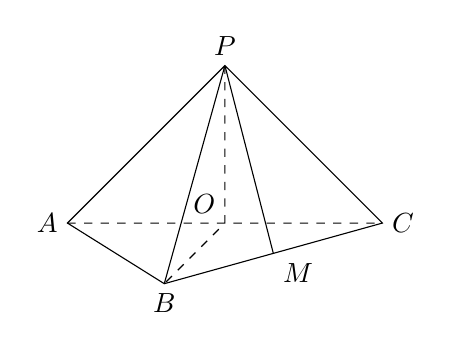
\begin{tikzpicture}[>=latex]
\draw (0,0,0) node [above left] {$O$} coordinate (O);
\draw (2,0,0) node [right] {$C$} coordinate (C);
\draw (-2,0,0) node [left] {$A$} coordinate (A);
\draw (0,0,2) node [below] {$B$} coordinate (B);
\draw (0,2,0) node [above] {$P$} coordinate (P);
\draw ($(B)!0.5!(C)$) node [below right] {$M$} coordinate (M);
\draw (A) -- (P) -- (C) -- (B) -- cycle (P) -- (B) (P) -- (M);
\draw [dashed] (A) -- (C) (P) -- (O) -- (B);
\end{tikzpicture}
\end{center}
(1) 求证: $PO\perp$平面$ABC$;\\
(2) 求直线$PM$与平面$PBO$所成的角的大小.
\item 将关于$x$的函数$y=\dfrac{m(x+2)^2}x$($m\in \mathbf{R}$)的图像向右平移$2$个单位后得到的函数图像记为$C$, 并设$C$所对应的函数为$f(x)$.\\
(1) 当$m>0$时, 试直接写出函数$f(x)$的单调递减区间;\\
(2) 设$f(4)=8$, 若函数$g(x)=x^2-2ax+5$($a>1$)对于任意$t_1\in [0, 1]$, 总存在$t_2\in [0, 1]$, 使得$g(t_2)=f (t_1)$成立, 求$a$的取值范围.
\item 某工厂制作如图所示的一种标识, 在半径为$R$的圆内作一个关于圆心对称的 ``H''型图形, ``H''型图形由两竖一横三个等宽的矩形组成, 两个竖直的矩形全等且它们的长边是横向矩形长边的$\dfrac{3}{2}$倍, 设$O$为圆心, $\angle AOB=2\alpha$, 记``H''型图形的面积为$S$.
\begin{center}
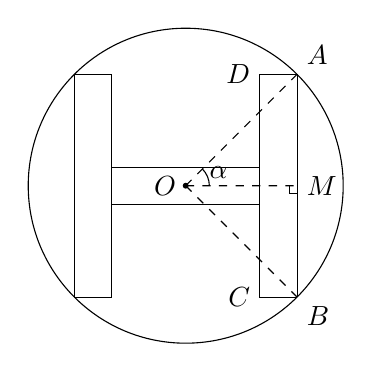
\begin{tikzpicture}[>=latex]
\draw (0,0) circle (2) node [left] {$O$} coordinate (O);
\filldraw (0,0) circle (0.03);
\draw (45:2) node [above right] {$A$} coordinate (A);
\draw (-45:2) node [below right] {$B$} coordinate (B);
\draw ($(A)!0.5!(B)$) node [right] {$M$} coordinate (M);
\draw [dashed] (O) -- (M) (O) -- (A) (O) -- (B);
\draw (O) pic ["$\alpha$",draw,angle eccentricity = 1.5, scale = 0.6] {angle = M--O--A};
\draw (A) -- (B);
\draw (A) ++ ({-sqrt(2)/3},0) node [left] {$D$} coordinate (D);
\draw (B) ++ ({-sqrt(2)/3},0) node [left] {$C$} coordinate (C);
\draw (A) -- (D) -- (C) -- (B);
\draw (M) pic [draw,scale = 0.2] {right angle = O--M--B};
\draw ({sqrt(2)*2/3},{sqrt(2)/6}) -- ({-sqrt(2)*2/3},{sqrt(2)/6});
\draw ({sqrt(2)*2/3},{-sqrt(2)/6}) -- ({-sqrt(2)*2/3},{-sqrt(2)/6});
\draw (135:2) --++ ({sqrt(2)/3},0) --++ (0,{-2*sqrt(2)}) --++ ({-sqrt(2)/3},0) --cycle;
\end{tikzpicture}
\end{center}
(1) 将$AB,AD$用$R,\alpha$表示, 并将$S$表示成$\alpha$的函数;\\
(2) 为了突出``H''型图形, 设计时应使$S$尽可能大, 则当$\alpha$为何值时, $S$最大? 并求出$S$的最大值.
\item 已知椭圆$C$的方程为$\dfrac{x^2}2+y^2=1$.、、
(1) 设$M(x_M,y_M)$是椭圆$C$上的点, 证明: 直线$\dfrac{x_Mx}2+y_My=1$与椭圆$C$有且只有一个公共点;\\
(2) 过点$N(1,\sqrt 2)$作两条与椭圆只有一个公共点的直线, 公共点分别记为$A$、$B$, 点$N$在直线$AB$上的射影为点$Q$, 求点$Q$的坐标;\\
(3) 互相垂直的两条直线$l_1$与$l_2$相交于点$P$, 且$l_1$、$l_2$都与椭圆$C$只有一个公共点, 求证点$P$落在$x^2+y^2=3$上.
\item 若数列$\{a_n\}$满足``对任意正整数$i$, $j$, $i\ne j$, 都存在正整数$k$, 使得$a_k=a_i\cdot a_j$'', 则称数列$\{a_n\}$具有``性质$P$''.\\
(1) 判断各项均等于$a$的常数列是否具有``性质$P$'', 并说明理由;\\
(2) 若公比为$2$的无穷等比数列$\{a_n\}$具有``性质$P$'', 求首项$a_1$的值;\\
(3) 若首项$a_1=2$的无穷等差数列$\{a_n\}$具有``性质$P$'', 求公差$d$的值.

%zmj3
\item 设集合$A=\{1,2,3,4\}$, 集合$B=\{1,3,5,7\}$, 则$A\cap B=$\blank{50}.
\item 行列式$\begin{vmatrix}1 & 2 & 0 \\2 & 3 & 5 \\5 & 8 & 0\end{vmatrix}$的值为\blank{50}.
\item 函数$y=\dfrac{\cos ^2x+1}2$的最小正周期为\blank{50}.
\item 设$\mathrm{i}$是虚数单位, 复数$z$满足$(1+2\mathrm{i})z=|4+3\mathrm{i}|$, 则$z=$\blank{50}.
\item 若$\{a_n\}$是无穷等比数列, 首项$a_1=1$, 公比$q=\dfrac 13$, 则$\{a_n\}$各项的和$S=$\blank{50}.
\item 在$4$名男生, $4$名女生中随机选出$3$名学生参加某次活动, 则选出的学生中至多$1$名女生的概率为\blank{50}(结果用最简分数表示).
\item 实数$x,y$满足约束条件$\begin{cases}x+2y\le 4, \\ 2x+y\le 3, \\ x\ge 0, \\ y\ge 0, \end{cases}$ 目标函数$z=x+y$的最大值为\blank{50}.
\item 已知曲线$C_1$的参数方程为$\begin{cases}
x=\sqrt 3t-1,  \\ y=t+\sqrt 3,  \end{cases}$($t$是参数) 曲线$C_2$的参数方程为$\begin{cases} x=-2+\sqrt 5\cos \theta,   \\ y=\sqrt 5\sin \theta,   \end{cases}$($\theta$是参数) 则$C_1$和$C_2$的两个交点之间的距离为\blank{50}.
\item 数列$\{a_n\}$满足$a_1=1$, 且$a_n+a_{n+1}=3n+2$对任意$n\in \mathbf{N}^*$均成立, 则$a_{2022}=$\blank{50}.
\item 设$n\in \mathbf{N}^*$, 若$(2+\sqrt x)^n$的二项展开式中, 有理项的系数之和为$365$, 则$n=$\blank{50}.
\item 设$\overrightarrow a$、$\overrightarrow b$、$\overrightarrow c$是同一平面上的三个两两不同的单位向量. 若$(\overrightarrow a\cdot \overrightarrow b):(\overrightarrow b\cdot \overrightarrow c):(\overrightarrow c\cdot \overrightarrow a)=1:1:3$, 则$\overrightarrow a\cdot\overrightarrow b$的值为\blank{50}.
\item 设$n\in \mathbf{N}^*$, 圆$C_n:x^2+y^2=R_n^2$($R_n>0$)与$y$轴正半轴的交点为$M$, 与曲线$y=\sqrt x$的交点为$N(x_n,y_n)$, 直线$MN$与$x$轴的交点为$A(a_n,0)$.若数列$\{x_n\}$满足: $x_{n+1}=4x_n+3$, $x_1=3$. 则常数$p=$\blank{50}使数列$\{a_{n+1}-p\cdot a_n\}$成等比数列.
\item 不等式$\dfrac{x-1}{x-2}\le 0$的解集为\bracket{20}.
\fourch{$[1,2]$}{$[1,2)$}{$(-\infty,1]\cup [2,+\infty)$}{$(-\infty,1)\cup (2,+\infty)$}
\item 设$z$是复数, 则``$z$是虚数''是``$z^3$是虚数''的\bracket{20}.
\twoch{充分非必要条件}{必要非充分条件}{充要条件}{既不充分又不必要条件}
\item 设$F_1,F_2$是椭圆$\dfrac{x^2}9+\dfrac{y^2}4=1$的两焦点, $A$与$B$分别是该椭圆的右顶点与上顶点. $P$是该椭圆上的一个动点, $O$是坐标原点. 记$s=\overrightarrow{F_1P}\cdot \overrightarrow{F_2P}-2\overrightarrow{OP}^2$. 在动点$P$在第一象限内从$A$沿椭圆向左上方运动到$B$的过程中, $s$的大小的变化情况为\bracket{20}.
\fourch{逐渐变大}{逐渐变小}{先变大后变小}{先变小后变大}
\item 设$\{a_n\}$是$2022$项的实数数列, $\{a_n\}$中的每一项都不为零. $\{a_n\}$中任意连续$11$项$a_n,a_{n+1},\cdots ,a_{n+10}$的乘积是定值($n=1,2,3,\cdots ,2012$). 命题\\
\textcircled{1} 不存在满足条件的数列, 使得其中恰有$365$个$1$;\\
\textcircled{2} 存在满足条件的数列, 使得其中恰有$550$个$1$;\\
的真假情况为\bracket{20}.
\twoch{\textcircled{1}和\textcircled{2}都是真命题}{\textcircled{1}是真命题, \textcircled{2} 是假命题}{\textcircled{2}是真命题, \textcircled{1} 是假命题}{\textcircled{1}和\textcircled{2}都是假命题}
\item 如图, 线段$OA$和$OB$是以$P$为顶点的圆锥的底面上的两条相互垂直的半径. 点$M$是母线$BP$的中点. 已知$OA=OM=2$.
\begin{center}
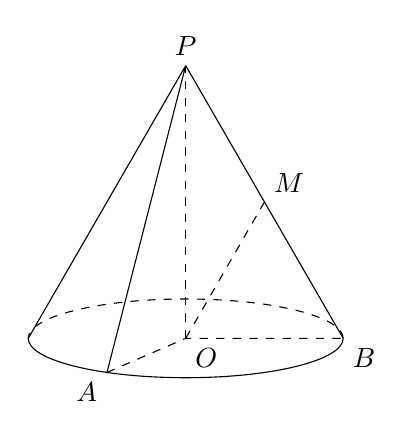
\begin{tikzpicture}[>=latex]
\draw (0,0) node [below right] {$O$} coordinate (O);
\draw (2,0) node [below right] {$B$} coordinate (B);
\draw (B) arc (0:-180:2 and 0.5);
\draw [dashed] (B) arc (0:180:2 and 0.5);
\draw [dashed] (O) --++ (0,{2*sqrt(3)}) node [above] {$P$} coordinate (P);
\draw ($(P)!0.5!(B)$) node [above right] {$M$} coordinate (M);
\draw ({2*cos(-120)},{0.5*sin(-120)}) node [below left] {$A$} coordinate (A);
\draw (P) -- (-2,0) (P) -- (A) (P) -- (B);
\draw [dashed] (A) -- (O) -- (B) (O) -- (M);
\end{tikzpicture}
\end{center}
(1) 求该圆锥的体积;\\
(2) 求异面直线$OM$与$AP$所成的角的大小.
\item 已知三角形$ABC$中, 三个内角$ABC$的对应边分别为$a$、$b$、$c$, 且$a=5$, $b=7$.\\
(1) 若$B=\dfrac{\pi}3$, 求$c$;\\
(2) 设点$M$是边$AB$的中点, 若$CM=3$, 求三角形$ABC$的面积.
\item 某地出现了虫害. 农业科学家引入了``虫害指数''数列$\{I_n\}$, $\{I_n\}$表示第$n$周的虫害的严重程度, 虫害指数越大, 严重程度越高. 为了治理虫害, 需要环境整治、杀灭害虫, 然而由于人力资源有限, 每周只能采取以下两个策略之一:\\
策略A: 环境整治, ``虫害指数''数列满足$I_{n+1}=1.02I_n-0.20$;\\
策略B: 杀灭害虫, ``虫害指数''数列满足$I_{n+1}=1.08I_n-0.46$;\\
当某周``虫害指数''小于$1$时, 危机就在这周解除.\\
(1) 设第一周的虫害指数$I_1\in [1,8]$, 用哪一个策略将使第二周的虫害的严重程度更小?\\
(2) 设第一周的虫害指数$I_1=3$, 如果每周都采用最优的策略, 虫害的危机最快在第几周解除?
\item 已知双曲线$H:x^2-\dfrac{y^2}{b^2}=1$($b>0$), 经过点$D(2,0)$的直线$l$与该双曲线交于$M$、$N$两点.\\
(1) 若$l$与$x$轴垂直, 且$|MN|=6$, 求$b$的值;\\
(2) 若$b=\sqrt 2$, 且$M$、$N$的横坐标之和为$-4$, 证明: $\angle MON=90^\circ$;\\
(3) 设直线$l$与$y$轴交于点$E$, $\overrightarrow{EM}=\lambda \cdot \overrightarrow{MD}$, $\overrightarrow{EN}=\mu \cdot \overrightarrow{ND}$, 求证: $\lambda +\mu$为定值.
\item $f(x)=2^{x+m}+m x+1$, 其中$m$是实常数.\\
(1) 若$f(\dfrac 1m)>18$, 求$m$的取值范围;\\
(2) 若$m>0$, 求证: 函数$f(x)$的零点有且仅有一个;\\
(3) 若$m>0$, 设函数$y=f(x)$的反函数为$y=f^{-1}(x)$, 若$a_1,a_2,a_3,a_4$是公差$d>0$的等差数列且均在函数$f(x)$的值域中, 求证: $f^{-1}(a_1)+f^{-1}(a_4)<f^{-1}(a_2)+f^{-1}(a_3)$.

%zmj4
\item 已知集合$U=\{-1,0,1,2,3\}$, $A=\{-1,0,2\}$, 则$\overline{A}=$\blank{50}.
\item 已知一个关于$x$、$y$的二元一次方程组的增广矩阵是$\begin{pmatrix}
1 & -1 & 1  \\ 0 & 1 & 2  \end{pmatrix}$, 则$x+y=$\blank{50}.
\item $\mathrm{i}$是虚数单位, 若复数$(1-2\mathrm{i})(a+\mathrm{i})$是纯虚数, 则实数$a$的值为\blank{50}.
\item 已知二项式$(x^2+\dfrac ax)^6$的展开式中含$x^3$项的系数是$160$, 则实数$a$的值是\blank{50}.
\item 直线$l$的参数方程为$\begin{cases} x=1+t, \\ y=-1+2t \end{cases}$($t$为参数), 则$l$的一个法向量为\blank{50}.
\item 已知某圆锥的主视图是边长为$2$的等边三角形, 则该圆锥的体积等于\blank{50}.
\item 已知椭圆$\dfrac{x^2}{a^2}+y^2=1$($a>0$)的左右焦点分别为$F_1$、$F_2$, 抛物线$y^2=2x$的焦点为$F$, 若$\overrightarrow{F_1F}=3\overrightarrow{FF_2}$, 则$a=$\blank{50}.
\item 甲、乙、丙、丁$4$名同学参加志愿者服务, 分别到三个路口疏导交通, 每个路口有$1$名或$2$名志愿者. 若每种分配方案的可能性相等, 则甲、乙两人在同一路口的概率为\blank{50}.
\item 将函数$f(x)=\sin x$的图像向右平移$\varphi$($\varphi >0$)个单位后得到函数$y=g(x)$的图像. 若对满足$|f(x_1)-g(x_2)|=2$的任意$x_1$、$x_2$, $|x_1-x_2|$的最小值是$\dfrac{\pi }3$, 则$\varphi$的最小值是\blank{50}.
\item 如图, 已知$AB$是边长为$1$的正六边形的一条边,
$P$在正六边形内(含边界), 则$\overrightarrow{AP}\cdot \overrightarrow{BP}$的取值范围是\blank{50}.
\begin{center}
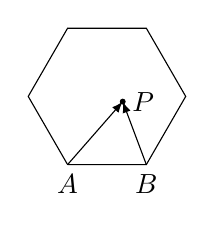
\begin{tikzpicture}[>=latex]
\draw (0,0) node [below] {$A$} coordinate (A) --++ (1,0) node [below] {$B$} coordinate (B) --++ (60:1) --++ (120:1) --++ (180:1) --++ (240:1) --++ (300:1);
\filldraw (0.7,0.8) circle (0.03) node [right] {$P$} coordinate (P);
\draw [->] (A) -- (P);
\draw [->] (B) -- (P);
\end{tikzpicture}
\end{center}
\item 已知曲线$C:y=\dfrac 2x$($1\le x\le 2$), 若对于曲线$C$上的任意一点$P(x,y)$, 都有$(x+y+c_1)(x+y+c_2)\le 0$, 则$|c_1-c_2|$的最小值为\blank{50}.
\item 在数列$\{a_n\}$中, $a_1=3$, $a_{n+1}=1+a_1\cdot a_2\cdot a_3\cdots a_n$, 记$T_n$为数列$\{\dfrac 1{a_n}\}$的前$n$项和, 则$\displaystyle\lim_{n\to\infty} T_n=$\blank{50}.
\item 设$\overrightarrow a$、$\overrightarrow b$分别是两条异面直线$l_1$、$l_2$的方向向量, 向量$\overrightarrow a$、$\overrightarrow b$夹角的取值范围为$A$, $l_1$、$l_2$所成角的取值范围为$B$, 则``$\alpha \in A$''是``$\alpha \in B$''的\bracket{20}.
\twoch{充要条件}{充分不必要条件}{必要不充分条件}{既不充分也不必要条件}
\item 若等比数列$\{a_n\}$的公比为$q$, 则关于$x$、$y$的二元一次方程组$\begin{cases} a_1x+a_5y=2, \\ a_2x+a_6y=1 \end{cases}$的解的情况下列说法正确的是\bracket{20}.
\twoch{对任意$q\in \mathbf{R}$($q\ne 0$), 方程组有唯一解}{对任意$q\in \mathbf{R}$($q\ne 0$), 方程组都无解}{当且仅当$q=\dfrac 12$时, 方程组有无穷多解}{当且仅当$q=\dfrac 12$时, 方程组无解}
\item 已知实数$a$、$b$满足$(a+2)(b+1)=8$, 有结论:\\
\textcircled{1} 当$a>0$, $b>0$时, $ab$存在最大值;\\
\textcircled{2} 当$a<0$, $b<0$时, $ab$存在最小值. 正确的判断是\bracket{20}.
\fourch{\textcircled{1}成立, \textcircled{2}成立}{\textcircled{1}不成立, \textcircled{2}不成立}{\textcircled{1}成立, \textcircled{2}不成立}{\textcircled{1}不成立, \textcircled{2}成立}
\item 已知函数$f(x)=\dfrac 1x+|2x-a|$. 若存在相异的实数$x_1,x_2\in (-\infty ,0)$, 使得$f(x_1)=f(x_2)$成立, 则实数$a$的取值范围为\bracket{20}.
\fourch{$(-\infty,-\dfrac{\sqrt{2}}2)$}{$(-\infty,-\sqrt{2})$}{$(\dfrac{\sqrt{2}}2,+\infty)$}{$(\sqrt 2,+\infty)$}
\item 已知在直三棱柱$ABC-A_1B_1C_1$中, $\angle BAC=90^\circ$, $AB=BB_1=1$, 直线$B_1C$与平面$ABC$成$30^\circ$的角.
\begin{center}
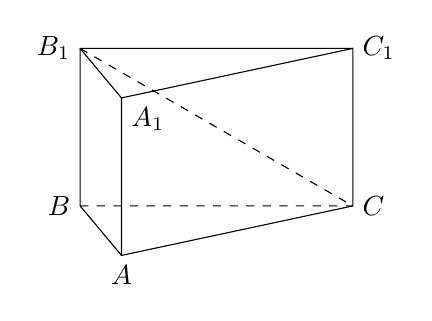
\begin{tikzpicture}[>=latex,scale = 2]
\draw (0,0,0) node [left] {$B$} coordinate (B);
\draw ({sqrt(3)},0,0) node [right] {$C$} coordinate (C);
\draw ($(B)!{1/3}!(C)$) ++ (0,0,{sqrt(2)/sqrt(3)}) node [below] {$A$} coordinate (A);
\draw (B) -- (A) -- (C) --++ (0,1) node [right] {$C_1$} coordinate (C1) --++ ({-sqrt(3)},0) node [left] {$B_1$} coordinate (B1) -- cycle;
\draw (A) --++ (0,1) node [below right] {$A_1$} coordinate (A1) -- (B1) (A1) -- (C1);
\draw [dashed] (B1) -- (C) (B) -- (C);
\end{tikzpicture}
\end{center}
(1)	求三棱锥$C_1-AB_1C$的体积;\\
(2) 求二面角$B-B_1C-A$的余弦值.
\item 已知复数$z$满足$|z|=\sqrt 2$, $z^2$的虚部为$2$.\\
(1) 求复数$z$;\\
(2) 设复数$z,z^2,z-z^2$在复平面上对应的点分别为$A,B,C$, 求: $(\overrightarrow{OA}+\overrightarrow{OB})\cdot \overrightarrow{OC}$的值.
\item 某公园内有一块以$O$为圆心半径为$20$米的圆形区域. 为丰富市民的业余文化生活, 现提出如下设计方案: 如图, 在圆形区域内搭建露天舞台, 舞台为扇形$OAB$区域, 其中两个端点$A$, $B$分别在圆周上; 观众席为等腰梯形$ABQP$内且在圆$O$外的区域, 其中$AP=AB=BQ$, $\angle PAB=\angle QBA=\dfrac{2\pi}3$, 且$AB,PQ$在点$O$的同侧. 为保证视听效果, 要求观众席内每一个观众到舞台中心$O$处的距离都不超过$60$米(即要求$PO\le 60$). 设$\angle OAB=\alpha$, $\alpha \in (0, \dfrac{\pi}3)$.
\begin{center}
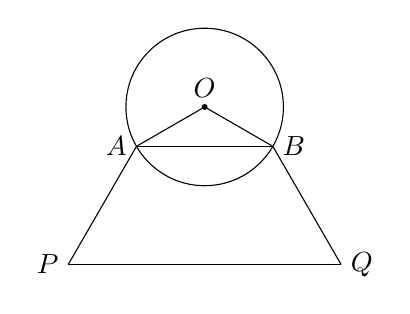
\begin{tikzpicture}[>=latex]
\draw (0,0) circle (1) node [above] {$O$} coordinate (O);
\filldraw (0,0) circle (0.03);
\draw (O) --++ (-30:1) node [right] {$B$} coordinate (B);
\draw (O) --++ (-150:1) node [left] {$A$} coordinate (A);
\draw (A) -- (B);
\draw (A) --++ (-120:{sqrt(3)}) node [left] {$P$} coordinate (P);
\draw (B) --++ (-60:{sqrt(3)}) node [right] {$Q$} coordinate (Q);
\draw (P) -- (Q);
\end{tikzpicture}
\end{center}
(1) 当$\alpha =\dfrac{\pi}6$时, 求舞台表演区域的面积;\\
(2) 对于任意$\alpha$, 上述设计方案是否均能符合要求?
\item 双曲线$C:x^2-\dfrac{y^2}{b^2}=1$($b>0$)的左顶点为$A$, 右焦点为$F$, 点$B$是双曲线$C$上一点.\\
(1) 当$b=2$时, 求双曲线两条渐近线的夹角;\\
(2) 若直线$BF$的倾斜角为$\dfrac{\pi}4$, 与双曲线$C$的另一交点为$D$, 且$|BD|=8$, 求$b$的值;\\
(3) 若$\overrightarrow{AF}\cdot \overrightarrow{BF}=0$, 且$|\overrightarrow{AF}|=|\overrightarrow{BF}|$, 点$E$是双曲线$C$上位于第一象限的动点, 求证: $\angle EFA=2\angle EAF$.
\item 设数列$\{a_n\}$的前$n$项和为$S_n$, 若$\dfrac 12\le \dfrac{a_{n+1}}{a_n}\le 2$($n\in \mathbf{N}^*$), 则称$\{a_n\}$是``紧密数列''.\\
(1) 已知数列$\{a_n\}$是``紧密数列'', 其前$5$项依次为$1,\dfrac 32,\dfrac 94,x,\dfrac{81}{16}$, 求$x$的取值范围;\\
(2) 若数列$\{a_n\}$的前$n$项和为$S_n=\dfrac 14(n^2+3n)$($n\in \mathbf{N}^*$), 判断$\{a_n\}$是否是``紧密数列'', 并说明理由;\\
(3) 设$\{a_n\}$是公比为$q$的等比数列, 若$\{a_n\}$与$\{S_n\}$都是``紧密数列'', 求$q$的取值范围.

%zmj5
\item 行列式$\begin{vmatrix} 1 & 2 \\ 3 & 4 \end{vmatrix}$的值为\blank{50}.
\item 设集合$A=\{x|y=\sqrt {x-1}, \ x\in \mathbf{R}\}$, $B=\{y|y=\sqrt {1-x^2}, \ x\in \mathbf{R}\}$, 则$A\cap B=$\blank{50}.
\item 若函数$f(x)=1+\dfrac 1x$($x>0$)的反函数为$f^{-1}(x)$, 则不等式$f^{-1}(x)>2$的解集为\blank{50}.
\item 已知常数$a>0$, 双曲线$4x^2-y^2=1$的一条渐近线与直线$ax+y+1=0$垂直, 则	$a=$\blank{50}.
\item 以抛物线$y^2=4x$的焦点为圆心, 且与该抛物线的准线相切的圆的标准方程	为\blank{50}.
\item 若$\log_ab=-2$, 则$a^2+b$的取值范围为\blank{50}.
\item 在一个水平放置的底面半径为$\sqrt 3$的的圆柱形量杯中装有适量的水, 现放入一个半径为$R$的实心铁球, 球完全浸没入水中且无水溢出. 若水面上升高度也为$R$, 则	$R=$\blank{50}.
\item 若$\alpha \in (\dfrac{\pi}4,\dfrac{\pi}2)$, $\sin 2\alpha =\dfrac 1{16}$, 则$\cos \alpha -\sin \alpha =$\blank{50}.
\item 在平面直角坐标系$xOy$中, 将点$A(2,1)$绕原点$O$逆时针旋转$\dfrac{\pi}4$到点$B$. 设直线$OB$的倾	斜角为$\alpha$, 则$\cos \alpha =$\blank{50}.
\item 已知数列$\{a_n\}$满足$a_{n+1}+a_n=4n+2$. 若$\{a_n\}$单调递增, 则$a_1$的取值范围为\blank{50}.
\item 已知复数$z_1,z_2$满足$|z_1|\le 1$, $-1\le \text{Re}z_2\le 1$, $-1\le \mathrm{Im}z_2\le 1$. 设$z=z_1+z_2$, 则$z$在复平面	上对应的点组成的图形的面积为\blank{50}.
\item 已知椭圆$\Gamma:\dfrac{x^2}2+y^2=1$的左、右焦点分别为$F_1,F_2$, 点$A$为椭圆$\Gamma$的上顶点, 坐标平面内的动点$P$满足$|AP|^2=2\overrightarrow{PF_1}\cdot \overrightarrow{PF_2}$, 则$|\overrightarrow{PF_1}+2\overrightarrow{PF_2}|$的最大值为\blank{50}.
\item 若$\cos \alpha >0$, $\sin 2\alpha <0$, 则角$\alpha$的终边所在象限是\bracket{20}.
\fourch{第一象限}{第二象限}{第三象限}{第四象限}
\item 过抛物线$y^2=8x$的焦点作直线与抛物线相交于两点, 且这两点的横坐标之和$9$, 则满足	条件的直线\bracket{20}.
\fourch{有$1$条}{有$2$条}{有无穷多条}{不存在}
\item 在$(\sqrt x+\dfrac 2{x^2})^n$($n\in \mathbf{N}^*$)的展开式中, 设含有$(\sqrt x)^{n-r}(\dfrac 2{x^2})^r$的项为第$r+1$($0\le r\le n$, $n\in \mathbf{N}$)项. 若第$3$项与第$5$项的系数之比为$3:56$, 则展开式中的常数项为\bracket{20}.
\fourch{$180$}{$160$}{$120$}{$100$}
\item 已知等差数列$\{a_n\}$与等比数列$\{b_n\}$都不是常数列. 设集合$S=\{k|a_k=b_k, \ k\in \mathbf{N}^*\}$, 则$S$	元素个数的最大值为\bracket{20}.
\fourch{$2$}{$3$}{$4$}{$5$}
\item 如图, 在$\mathbf{R}t\triangle ABC$中, $AB\perp AC$. $PA\perp$平面$ABC$, $D$为$AC$的中点. 过点$D$作$DE\perp$平面$ABC$, $DE<AP$, 连结$BP,BE$.
\begin{center}
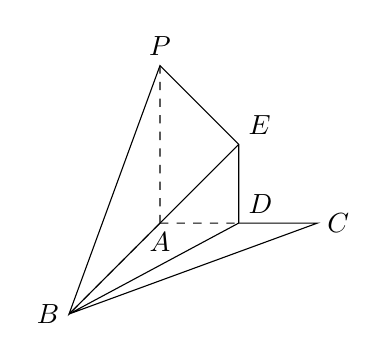
\begin{tikzpicture}[>=latex]
\draw (0,0,0) node [below] {$A$} coordinate (A);
\draw (1,0,0) node [above right] {$D$} coordinate (D);
\draw (2,0,0) node [right] {$C$} coordinate (C);
\draw (1,1,0) node [above right] {$E$} coordinate (E);
\draw (0,2,0) node [above] {$P$} coordinate (P);
\draw (0,0,3) node [left] {$B$} coordinate (B);
\draw (B) -- (D) -- (C) -- cycle;
\draw (D) -- (E) -- (P) -- (B) -- (E);
\draw [dashed] (A) -- (B) (A) -- (D) (A) -- (P);
\end{tikzpicture}
\end{center}
(1) 作出平面$PBE$与平面$ABC$的交线(保留作图痕迹);\\
(2) 若$PA=AC=2$, $DE=1$, 四棱锥$B-ADEP$的体积为$\dfrac{\sqrt 3}3$, 求平面$PBE$与平面$ABC$所成锐二面角的大小.
\item 设函数$f(x)=2\sin (x+\dfrac{\pi }3)\cos x$.\\
(1) 求$f(x)$在$[0,\dfrac{\pi }2]$上的值域;\\
(2) 记$\triangle ABC$三个内角$A,B,C$的对边分别为$a,b,c$. 若$A$为锐角, $f(A)=\dfrac{\sqrt 3}2$, $b=2$, $c=3$, 求$\cos (A-B)$的值.
\item 某企业参加$A$项目生产的工人为$1000$人, 平均每人每年创造利润$10$万元. 根据现实的需要, 从$A$项目中调出$x$人参与$B$项目的售后服务工作, 每人每年可以创造利润$10(a-\dfrac{3x}{500})$万元(其中常数$a>0$), $A$项目余下的工人每人每年创造利润需要提高$0.2x\%$.\\
(1) 若要保证$A$项目余下的工人创造的年总利润不低于原来$1000$名工人创造的年总利润, 则最多调出多少人参加$B$项目从事售后服务工作?\\
(2) 当从$A$项目调出的人数不超过总人数的$40\%$时, 总能使得$A$项目中留岗工人创造的年总利润不低于调出的工人所创造的年总利润, 求$a$的取值范围.
\item 已知常数$k>0$, 在平面直角坐标系$xOy$中, $A,B$两点分别在第一象限、第四象限, 直线$OA,OB$的一个方向向量分别为$\overrightarrow{d_1}=(1,k)$, $\overrightarrow{d_2}=(1,-k)$, 动点$P$在$\angle AOB$内, 过点$P$分别作$PM\perp OA$于$M$, $PN\perp OB$于$N$, $M,N$分别在射线$OA,OB$上.\\
(1) 若$k=1$, $P(\dfrac 32,\dfrac 12)$, 求$|OM|$的值;\\
(2) 若$P(2,1)$, $\triangle OMP$的面积为$\dfrac 65$, 求$k$的值;\\
(3) 设线段$MN$的中点为$T$. 当$\triangle MON$的面积为$\dfrac 1k$时, 求证: $|OT|\ge \dfrac 1k$.
\item 若无穷数列$\{a_n\}$满足: \textcircled{1} 存在互异的$p,q\in \mathbf{N}^*$使得$a_p=a_q$; \textcircled{2} 对任意$n\in \mathbf{N}^*$, 当$n\ne p$且$n\ne q$时, 恒有$a_n>a_p$, 则称$\{a_n\}$具有性质$P$.\\
(1) 已知常数$k\in \mathbf{N}^*$, 无穷数列$\{a_n\}$的通项公式为$a_n=n+\dfrac kn$. 若$\{a_n\}$具有性质$P$, 求$k$的值;\\
(2) 已知常数$\lambda \in \mathbf{R}$, 无穷数列$\{a_n\}$的通项公式为$a_n=\begin{cases} -2n+11, & 1\le n\le 5, \\ 2^{n-5}+\lambda, & n\ge 6. \end{cases}$若$\{a_n\}$具有性质$P$, 求$\lambda$的值以及$\{a_n\}$的前$n$项和$S_n$;\\
(3) 已知常数$t\in \mathbf{Z}$, 无穷数列$\{a_n\}$的通项公式为$a_n=(tn+3)(\dfrac 9{10})^n$. 问: 是否存在$t$, 使得$\{a_n\}$具有性质$P$? 若存在, 求出所有$t$的值; 若不存在, 说明理由.

%zmj6
\item $(x^2+\dfrac 1x)^8$的展开式中$x^4$项的系数是\blank{50}.
\item 设变量$x, y$满足约束条件$\begin{cases} 0\le x\le 1, \\ y\le 2, \\ x\le y.\end{cases}$则$z=x+y$的最大值为\blank{50}.
\item 已知奇函数$y=f(x)$的周期为$2$, 且当$x\in (0,1]$时, $f(x)=\log_2 x$. 则$f(7.5)$的值为\blank{50}.
\item 一个几何体的三视图如图所示, 则这个几何体的表面积为\blank{50}.
\begin{center}
\begin{tikzpicture}[>=latex]
\draw (0,0) -- (2,0) -- (2,1) -- (0,1) -- cycle;
\draw (0,1) -- (1,2) -- (2,1);
\draw (-0.1,0) -- (-0.5,0) (-0.1,1) -- (-0.5,1) (0.9,2) -- (-0.5,2);
\draw [->] (-0.3,0.2) -- (-0.3,0);
\draw [->] (-0.3,0.8) -- (-0.3,1);
\draw (-0.3,0.5) node {$1$};
\draw [->] (-0.3,1.2) -- (-0.3,1);
\draw [->] (-0.3,1.8) -- (-0.3,2);
\draw (-0.3,1.5) node {$1$};
\draw (0,-0.1) -- (0,-0.5) (2,-0.1) -- (2,-0.5);
\draw [->] (0.8,-0.3) -- (0,-0.3);
\draw [->] (1.2,-0.3) -- (2,-0.3);
\draw (1,-0.3) node {$2$};
\draw (1,-0.8) node {主视图};
\draw (3,0) -- (5,0) -- (5,1) -- (3,1) -- cycle;
\draw (3,1) -- (4,2) -- (5,1);
\draw (2.9,0) -- (2.5,0) (2.9,1) -- (2.5,1) (3.9,2) -- (2.5,2);
\draw [->] (2.7,0.2) -- (2.7,0);
\draw [->] (2.7,0.8) -- (2.7,1);
\draw (2.7,0.5) node {$1$};
\draw [->] (2.7,1.2) -- (2.7,1);
\draw [->] (2.7,1.8) -- (2.7,2);
\draw (2.7,1.5) node {$1$};
\draw (3,-0.1) -- (3,-0.5) (5,-0.1) -- (5,-0.5);
\draw [->] (3.8,-0.3) -- (3,-0.3);
\draw [->] (4.2,-0.3) -- (5,-0.3);
\draw (4,-0.3) node {$2$};
\draw (4,-0.8) node {左视图};
\draw (1,-2.5) circle (1);
\draw (0.9,-1.5) -- (-0.5,-1.5) (0.9,-3.5) -- (-0.5,-3.5);
\draw [->] (-0.3,-2.2) -- (-0.3,-1.5);
\draw [->] (-0.3,-2.8) -- (-0.3,-3.5);
\draw (-0.3,-2.5) node {$2$};
\draw (0,-2.6) -- (0,-4) (2,-2.6) -- (2,-4);
\draw [->] (0.8,-3.8) -- (0,-3.8);
\draw [->] (1.2,-3.8) -- (2,-3.8);
\draw (1,-3.8) node {$2$};
\draw (1,-4.2) node {俯视图};
\filldraw (1,-2.5) circle (0.03);
\end{tikzpicture}
\end{center}
\item 投掷两颗六个面上分别刻有$1$到$6$的点数的均匀的骰子, 得到其向上的点数分别为$m$和$n$, 则复数$\dfrac{m+n\mathrm{i}}{n+m\mathrm{i}}$为虚数的概率为\blank{50}.
\item 某茶农打算在自己的茶园建造一个容积为$500$立方米的长方体无盖蓄水池, 要求池底面的长和宽之和为$20$米. 若每平方米的池底面造价是池侧壁的两倍, 则为了使蓄水池的造价最低, 蓄水池的高应该为\blank{50}米.
\item 如图, 在直角梯形$ABCD$中, $AD\parallel BC$, $\angle DC=90^\circ$, $AD=2$, $BC=1$, $P$为梯形的腰$DC$上的动点, 则
$|\overrightarrow{PA}+3\overrightarrow{PB}|$的最小值为\blank{50}.
\begin{center}
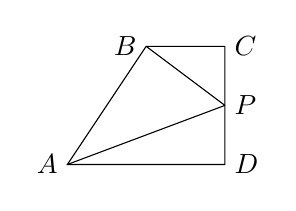
\begin{tikzpicture}[>=latex]
\draw (0,0) node [left] {$A$} coordinate (A) --++ (2,0) node [right] {$D$} coordinate (D) --++ (0,1.5) node [right] {$C$} coordinate (C) --++ (-1,0) node [left] {$B$} coordinate (B) -- cycle;
\draw (A) -- ($(C)!0.5!(D)$) node [right] {$P$} coordinate (P) (P) -- (B);
\end{tikzpicture}
\end{center}
\item 如图, 在正六棱柱的所有棱中任取两条, 则它们所在的直线是互相垂直的异面直线的概率为\blank{50}.
\begin{center}
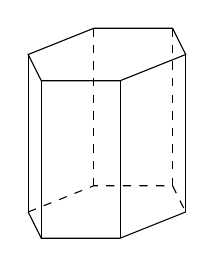
\begin{tikzpicture}[>=latex]
\draw (0,0,0) coordinate (A) --++ (1,0,0) coordinate (B) --++ ({1/2},0,{sqrt(3)/2}) coordinate (C) --++ ({-1/2},0,{sqrt(3)/2}) coordinate (D) --++ (-1,0,0) coordinate (E) --++ ({-1/2},0,{-sqrt(3)/2}) coordinate (F) -- cycle;
\draw [dashed] (A) --++ (0,-2,0) coordinate (A1);
\draw [dashed] (B) --++ (0,-2,0) coordinate (B1);
\draw (C) --++ (0,-2,0) coordinate (C1);
\draw (D) --++ (0,-2,0) coordinate (D1);
\draw (E) --++ (0,-2,0) coordinate (E1);
\draw (F) --++ (0,-2,0) coordinate (F1);
\draw (F1) -- (E1) -- (D1) -- (C1);
\draw [dashed] (F1) -- (A1) -- (B1) -- (C1);
\end{tikzpicture}
\end{center}
\item 已知双曲线$\dfrac{x^2}{a^2}-\dfrac{y^2}{b^2}=1$($a>0$, $b>0$)的两焦点分别为$F_1,F_2$, $P$为双曲线上一点, $PF_2\perp x$轴, 且$|PF_2|$是$|PF_1|$与$|F_1F_2|$的等差中项, 则双曲线的渐近线方程为\blank{50}.
\item 若四边形$ABCD$是边长为$4$的菱形, $P$为其所在平面上的任意点, 则$|\overrightarrow{PA}\cdot \overrightarrow{PC}-\overrightarrow{PB}\cdot \overrightarrow{PD}|$的取值范围是\blank{50}.
\item 已知函数$f(x)=\begin{cases}
\tan x, & x\in (-\dfrac{\pi }2,\dfrac{\pi }3]\cup (\dfrac{2\pi }3,\dfrac{3\pi }2),  \\ -\dfrac{6\sqrt 3}{\pi }x+3\sqrt 3, & x\in (\dfrac{\pi }3,\dfrac{2\pi }3].  \end{cases}$若$f(x)$在区间$D$上的最大值存在, 记该最大值为$K\{D\}$, 则满足等式$K\{[0,a)\}=3\cdot K\{[a,2a]\}$的实数$a$的取值集合是\blank{50}.
\item 已知数列$\{a_n\}$($n\in \mathbf{N}^*$)满足$a_{n+1}=|a_2-a_1|+|a_3-a_2|+\cdots +|a_n-a_{n-1}|$($n\ge 2$), 且$a_1=1$, $a_2=a$($a>1$), 则$a_1+a_2+a_3+\cdots +a_{24}=$\blank{50}. (结果用含$a$的式子表示)
\item 为客观了解上海市民家庭存书量, 上海市统计局社情民意调查中心通过电话调查系统开展专项调查, 成功访问了$2007$位市民. 在这项调查中, 总体、样本及样本的容量分别是\bracket{20}.
\onech{总体是上海市民家庭总数量, 样本是$2007$位市民家庭的存书量, 样本的容量是$2007$}{总体是上海市民家庭的存书量, 样本是$2007$位市民家庭的存书量, 样本的容量是$2007$}{总体是上海市民家庭的存书量, 样本是$2007$位市民, 样本的容量是$2007$}{总体是上海市民家庭总数量, 样本是$2007$位市民, 样本的容量是$2007$}
\item 某县共有$300$个村, 现采取系统抽样方法, 抽取15个村作为样本, 调查农民的生活和生产状况, 将$300$个村编上$1$到$300$的号码, 求得间隔数$k=\dfrac{300}{15}=20$, 即每$20$个村抽取一个村, 在$1$到$20$中随机抽取一个数字$7$, 则在$41$到$60$这$20$个数中应取得号码是\bracket{20}.
\fourch{$45$}{$46$}{$47$}{$48$}
\item 已知抛物线的方程为$y^2=4x$, 过其焦点$F$的直线交抛物线于$M,N$两点, 交$y$轴于点$E$, 若$\overrightarrow{EM}=\lambda _1\overrightarrow{MF},\overrightarrow{EN}=\lambda _2\overrightarrow{NF}$, 则$\lambda _1+\lambda _2=$\bracket{20}.
\fourch{$2$}{$-2$}{$1$}{$-1$}
\item 已知关于$x$的实系数方程: $x^2-4x+5=0$和$x^2+2mx+m=0$的四个不同的根, 若这四个根在复平面上对应的点共圆, 则$m$取值范围是\bracket{20}.
\fourch{$\{5\}$}{$\{-1\}$}{$(0,1)$}{$(0,1)\cup \{-1\}$}
\item 如图, 在直三棱柱$ABC-A_1BC_1$中, $AB\perp BC$, $AB=BC=2$, $AA_1=2\sqrt 3$, $M$是侧棱$C_1C$上一点, 设$MC=h$.
\begin{center}
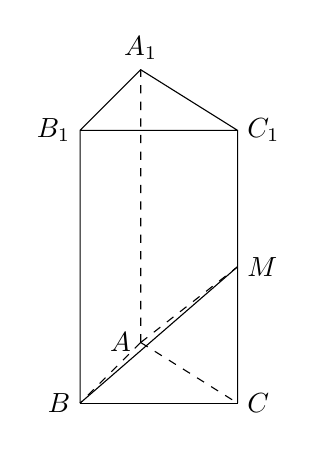
\begin{tikzpicture}[>=latex]
\draw (0,0,0) node [left] {$B$} coordinate (B) -- (2,0,0) node [right] {$C$} coordinate (C);
\draw (0,0,-2) node [left] {$A$} coordinate (A);
\draw (A) ++ (0,{2*sqrt(3)},0) node [above] {$A_1$} coordinate (A1);
\draw (B) ++ (0,{2*sqrt(3)},0) node [left] {$B_1$} coordinate (B1);
\draw (C) ++ (0,{2*sqrt(3)},0) node [right] {$C_1$} coordinate (C1);
\draw (B) -- (B1) -- (A1) -- (C1) -- (C) (B1) -- (C1);
\draw [dashed] (A) -- (A1) (A) -- (B) (A) -- (C);
\draw ($(C)!0.5!(C1)$) node [right] {$M$} coordinate (M);
\draw (M) -- (B);
\draw [dashed] (A) -- (M);
\end{tikzpicture}
\end{center}
(1) 若$h=\sqrt 3$, 求多面体$ABM-A_1B_1C_1$的体积;\\
(2) 若异面直线$BM$与$A_1C_1$所成的角为$60^{^\circ}$, 求$h$的值.
\item 已知函数$f(x)=3\cos ^2\omega x+\sqrt 3\sin \omega x\cos \omega x$($\omega >0$).\\
(1) 当$f(x)$的最小正周期为$2\pi$时, 求$\omega$的值;\\
(2) 当$\omega =1$时, 设三角形$\triangle ABC$的内角$A,B,C$对应的边分别为$a,b,c$, 已知$f(\dfrac A2)=3$, 且$a=2\sqrt 7$, $b=6$, 求$\triangle ABC$的面积.
\item 如图, $AB$两地相距$100$公里, 两地政府为提升城市的抗疫能力, 决定在$AB$之间选址$P$点建造储备仓库, 共享民生物资, 当点$P$在线段$AB$的中点$C$时, 建造费用为$2000$万元; 若点$P$在线段$AC$上(不含点$A$), 则建造费用与$PA$之间的距离成反比; 若点$P$在线段$CB$上(不含点$B$), 则建造费用与$PB$之间的距离成反比, 现假设$PA$之间的距离为$x$千米$(0<x<100)$, $A$地所需该物资每年的运输费用为$2.5x$万元, $B$地所需该物资每年的运输费用为$0.5(100-x)$万元, $f(x)$表示建造仓库费用, $g(x)$表示两地物资每年的运输总费用(单位: 万元).
\begin{center}
\begin{tikzpicture}[>=latex]
\filldraw (0,0) node [left] {$A$} coordinate (A) circle (0.03);
\filldraw (4,0) node [below] {$C$} coordinate (C) circle (0.03);
\filldraw (8,0) node [right] {$B$} coordinate (B) circle (0.03);
\draw (2,0) node [below] {$50$千米} (6,0) node [below] {$50$千米};
\filldraw (2.5,0) circle (0.03) node [above] {$P$};
\draw (A) -- (B);
\end{tikzpicture}
\end{center}
(1) 求函数$f(x)$的解析式;\\
(2) 若规划仓库使用的年数为$n$($n\in \mathbf{N}^*)$,$H(x)=f(x)+ng(x)$, 求$H(x)$的最小值, 并解释其何处取得最小值的实际意义.
\item 已知椭圆$\Gamma :\dfrac{x^2}4+y^2=1$的左右顶点分别为$AB$, $P$是椭圆$\Gamma$上异于$AB$的一点, 直线$l:x=4$, 直线$AP,BP$分别交直线$l$于两点$C,D$, 线段$CD$的中点为$E$.
\begin{center}
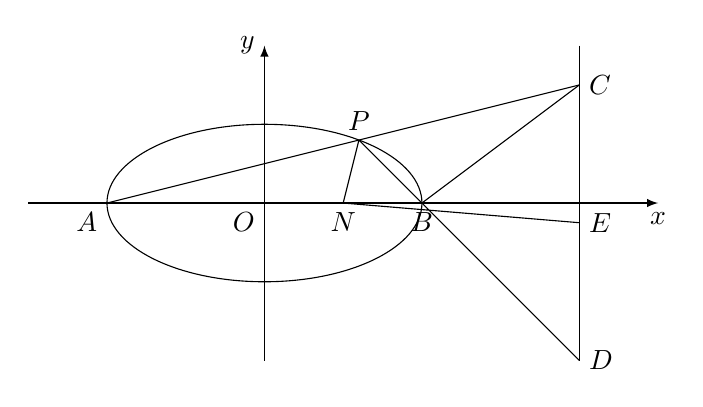
\begin{tikzpicture}[>=latex]
\draw [->] (-3,0) -- (5,0) node [below] {$x$};
\draw [->] (0,-2) -- (0,2) node [left] {$y$};
\draw (0,0) node [below left] {$O$};
\draw (4,2) -- (4,-2);
\draw (0,0) ellipse (2 and 1);
\draw (-2,0) node [below left] {$A$} coordinate (A) (2,0) node [below] {$B$} coordinate (B);
\draw (1.2,0.8) node [above] {$P$} coordinate (P);
\draw ($(A)!{6/3.2}!(P)$) node [right] {$C$} coordinate (C);
\draw ($(P)!{2.8/0.8}!(B)$) node [right] {$D$} coordinate (D);
\draw ($(C)!0.5!(D)$) node [right] {$E$} coordinate (E);
\draw (1,0) node [below] {$N$} coordinate (N);
\draw (P) -- (N) -- (E) (A) -- (C) (P) -- (D);
\draw (B) -- (C);
\end{tikzpicture}
\end{center}
(1) 设直线$AP,BP$的斜率分别为$k_{AP},k_{BP}$, 求$k_{AP}\cdot k_{BP}$的值;\\
(2) 设$\triangle ABP, \triangle ABC$的面积分别为$S_1S_2$, 如果$S_2=2S_1$, 求直线$AP$的方程;\\
(3) 在$x$轴上是否存在定点$N(n,0)$, 使得当直线$NP,NE$的斜率$k_{NP},k_{NE}$存在时, $k_{NP}\cdot k_{NE}$为定值? 若存在, 求出$k_{NP}\cdot k_{NE}$的值; 若不存在, 请说明理由.
\item 对于有限集$S=\{a_1,a_2,a_3,\cdots ,a_{m-1},a_m\}$($m\in \mathbf{N}^*$, $m\ge 3$), 如果存在函数$f(x)$($f(x)=x$除外), 其图像在区间$D$($S\subseteq D$)上是一段连续曲线, 且满足$f(S)=S$, 其中$f(S)=\{f(x)|x \in S\}$, 那么称这个函数$f(x)$是$P$变换, 集合$S$是$P$集合, 数列$a_1,a_2,a_3,\cdots ,a_{m-1},a_m$是$P$数列.\\
例如, $S=\{1,2,3\}$是$P$集合, 此时函数$f(x)=4-x$是$P$变换, 数列$1,2,3$或$3,2,1$等都是$P$数列.\\
(1) 判断数列$1,2,5,8,9$是否是$P$数列? 说明理由;\\
(2) 若各项均为正数的递增数列$\{a_n\}$($1\le n\le 2021$, $n\in \mathbf{N}^*$)是$P$数列, 若$P$变换$f(x)=\dfrac 9x$, 求$a_1\cdot a_2\cdot \cdots \cdot a_{2021}$的值;\\
(3) 元素都是正数的有限集$S=\{a_1,a_2,a_3,\cdots ,a_{m-1},a_m\}$($m\in \mathbf{N}^*$, $m\ge 3$), 若$a_i<a_j$, 总有$\dfrac{a_j}{a_i}\in S$, 其中$1\le i,j\le m$. 试判断集合$S$是否是$P$集合? 请说明理由.

%zmj7
\item 已知集合$A=\{1, 2, m\}$, $B=\{2, 4\}$, 若$A\cup B=\{1, 2, 3, 4\}$, 则实数$m=$\blank{50}.
\item $(x+\dfrac 1x)^n$的展开式中的第$3$项为常数项, 则正整数$n=$\blank{50}.
\item 已知复数$z$满足$z^2=4+3\mathrm{i}$($\mathrm{i}$为虚数单位), 则$|z|=$\blank{50}.
\item $\displaystyle\lim_{n\to \infty} \dfrac{2^{n+1}+3^{n+1}}{2^n+3^n}=$\blank{50}.
\item 若圆锥的侧面积是底面积的$2$倍, 则其母线与轴所成角的大小是\blank{50}.
\item 设变量$x$、$y$满足条件$\begin{cases} x\ge 1,\\ x+y-4\le 0,\\ x-3y+4\le 0,\end{cases}$则目标函数$z=3x-y$的最大值为\blank{50}.
\item 直线$\begin{cases} x=2+t,\\ y=4-t, \end{cases}$($t$为参数)与曲线$\begin{cases} x=3+\sqrt 2\cos \theta ,\\ y=5+\sqrt 2\sin \theta,  \end{cases}$($\theta$为参数)的公共点的个数是\blank{50}.
\item 若$f(x)=x^{\frac 13}-x^{-\frac 12}$, 则满足$f(x)>0$的$x$的取值范围是\blank{50}.
\item 某商场举行购物抽奖促销活动, 规定每位顾客从装有编号为$0$、$1$、$2$、$3$的四个相同小球的抽奖箱中, 每次取出一球记下编号后放回, 连续取两次, 若取出的两个小球编号相加之和等于$6$, 则中一等奖, 等于$5$中二等奖, 等于$4$或$3$中三等奖. 则顾客抽奖中三等奖的概率为\blank{50}.
\item 已知函数$f(x)=\lg (\sqrt {x^2+1}+ax)$的定义域为$\mathbf{R}$, 则实数$a$的取值范围是\blank{50}.
\item 在$\triangle ABC$中, $M$是$BC$的中点, $\angle A=120^\circ$, $\overrightarrow{AB}\cdot \overrightarrow{AC}=-\dfrac 12$, 则线段$AM$长的最小值为\blank{50}.
\item 若实数$x$、$y$满足$4^x+4^y=2^{x+1}+2^{y+1}$, 则$S=2^x+2^y$的取值范围是\blank{50}.
\item 命题``若$x=1$, 则$x^2-3x+2=0$''的逆否命题是\bracket{20}.
\twoch{若$x\ne 1$, 则$x^2-3x+2\ne 0$}{若$x^2-3x+2=0$, 则$x=1$}{若$x^2-3x+2=0$, 则$x\ne 1$}{若$x^2-3x+2\ne 0$, 则$x\ne 1$}
\item 某单位现有职工$52$人, 将所有职工编号, 用系统抽样的方法抽取一个容量为$4$的样本. 已知$6$号、$32$号、$45$号职工在样本中, 则另一个在样本中的职工编号为\bracket{20}.
\fourch{$18$}{$19$}{$20$}{$21$}
\item 如图, 在正方体$ABCD-A_1B_1C_1D_1$中, $M$、$E$是$AB$的三等分点, $G$、$N$是$CD$的三等分点, $F$、$H$分别是$BC$、$MN$的中点, 则四棱锥$A_1-EFGH$的左视图是\bracket{20}.
\begin{center}
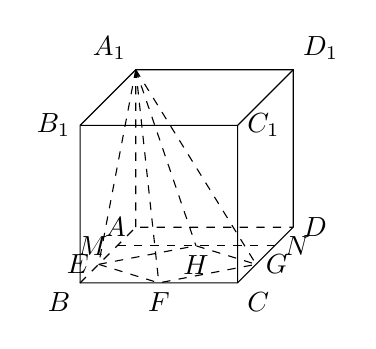
\begin{tikzpicture}[>=latex]
\draw (0,0) node [below left] {$B$} coordinate (B) --++ (2,0) node [below right] {$C$} coordinate (C) --++ (45:{2/2}) node [right] {$D$} coordinate (D)
--++ (0,2) node [above right] {$D_1$} coordinate (D1)
--++ (-2,0) node [above left] {$A_1$} coordinate (A1) --++ (225:{2/2}) node [left] {$B_1$} coordinate (B1) -- cycle;
\draw (B) ++ (2,2) node [right] {$C_1$} coordinate (C1) -- (C) (C1) --++ (45:{2/2}) (C1) --++ (-2,0);
\draw [dashed] (B) --++ (45:{2/2}) node [left] {$A$} coordinate (A) --++ (2,0) (A) --++ (0,2);
\draw [dashed] ($(A)!{1/3}!(B)$) node [left] {$M$} coordinate (M) -- ($(D)!{1/3}!(C)$) node [right] {$N$} coordinate (N);
\draw [dashed] ($(A)!{2/3}!(B)$) node [left] {$E$} coordinate (E) -- ($(B)!0.5!(C)$) node [below] {$F$} coordinate (F)--($(D)!{2/3}!(C)$) node [right] {$G$} coordinate (G);
\draw [dashed] (E) -- ($(M)!0.5!(N)$) node [below] {$H$} coordinate (H) -- (G);
\draw [dashed] (A1) -- (E) (A1) -- (F) (A1) -- (G) (A1) -- (H);
\end{tikzpicture}
\end{center}

\fourch{\begin{center}
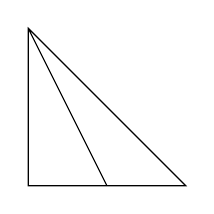
\begin{tikzpicture}[>=latex]
\draw (0,0) -- (2,0) -- (0,2) -- cycle (1,0) -- (0,2);
\end{tikzpicture}
\end{center}}{\begin{center}
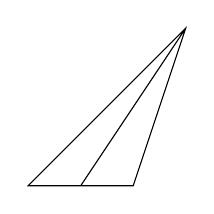
\begin{tikzpicture}[>=latex]
\draw (0,0) -- ({4/3},0) -- (2,2) -- cycle ({2/3},0) -- (2,2);
\end{tikzpicture}
\end{center}}{
\begin{center}
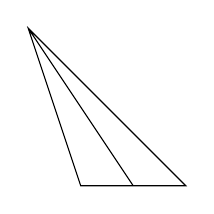
\begin{tikzpicture}[>=latex]
\draw ({2/3},0) -- (2,0) -- (0,2) -- cycle ({4/3},0) -- (0,2);
\end{tikzpicture}
\end{center}
}{\begin{center}
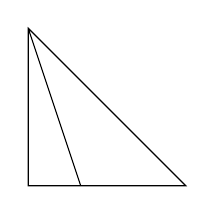
\begin{tikzpicture}[>=latex]
\draw (0,0) -- (2,0) -- (0,2) -- cycle ({2/3},0) -- (0,2);
\end{tikzpicture}
\end{center}}
\item 在某种计算机语言中, 有一种函数$y=\texttt{INT}(x)$叫做取整函数(也叫高斯函数), 它表示$y$等于不超过$x$的最大整数, 如$\texttt{INT}(0.9)=0$, $\texttt{INT}(3.14)=3$. 已知$a_n=\texttt{INT}(\dfrac 27\times 10^n)$, $b_1=a_1$, $b_n=a_n-10a_{n-1}$($n\in \mathbf{N}^*$且$n\ge 2$), 则$b_{2018}$等于\bracket{20}.
\fourch{$2$}{$5$}{$7$}{$8$}
\item 如图, 在四棱锥$P-ABCD$中, 底面$ABCD$为直角梯形, $\angle BAD=90^\circ$, $AD\parallel BC$, $AB=2$, $AD=1$, $PA=BC=4$, $PA\perp$平面$ABCD$.
\begin{center}
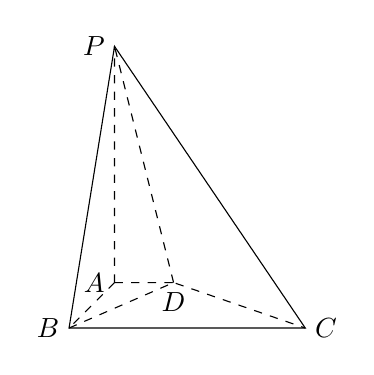
\begin{tikzpicture}[>=latex, scale = 0.75]
\draw (0,0,0) node [left] {$A$} coordinate (A);
\draw (0,4,0) node [left] {$P$} coordinate (P);
\draw (0,0,2) node [left] {$B$} coordinate (B);
\draw (1,0,0) node [below] {$D$} coordinate (D);
\draw (4,0,2) node [right] {$C$} coordinate (C);
\draw (B) -- (C) -- (P) -- cycle;
\draw [dashed] (A) -- (B) (A) -- (D) (A) -- (P) (B) -- (D) -- (C) (D) -- (P);
\end{tikzpicture}
\end{center}
(1) 求异面直线$BD$与$PC$所成角的大小;\\
(2) 求二面角$A-PC-D$的余弦值.
\item 在$\triangle ABC$中, 内角$A$、$B$、$C$所对的边分别为$a$、$b$、$c$, 已知$a-b=2$, $c=4$, $\sin A=2\sin B$.\\
(1) 求$\triangle ABC$的面积$S$;\\
(2) 求$\sin (2A-B)$的值.
\item 某创新团队拟开发一种新产品, 根据市场调查估计能获得$200$万元到$1000$万元的收益. 现准备制定一个奖励方案: 奖金$y$(单位: 万元)随收益$x$(单位: 万元)的增加而增加, 且奖金不超过$9$万元, 同时奖金不超过收益的$20\%$.\\
(1) 若建立函数$y=f(x)$模型制定奖励方案, 试用数学语言表述该团队对奖励函数$f(x)$模型的基本要求, 并分析函数$y=\dfrac x{150}+2$是否符合团队要求的奖励函数模型, 并说明原因;\\
(2) 若该团队采用模型函数$f(x)=\dfrac{10x-3a}{x+2}$作为奖励函数模型, 试求$a$的取值范围.
\item 已知椭圆$\Gamma$: $\dfrac{x^2}{a^2}+\dfrac{y^2}{b^2}=1$($a>b>0$)的焦距为$2\sqrt 3$, 点$P(0, 2)$关于直线$y=-x$的对称点在椭圆$\Gamma$上.
\begin{center}
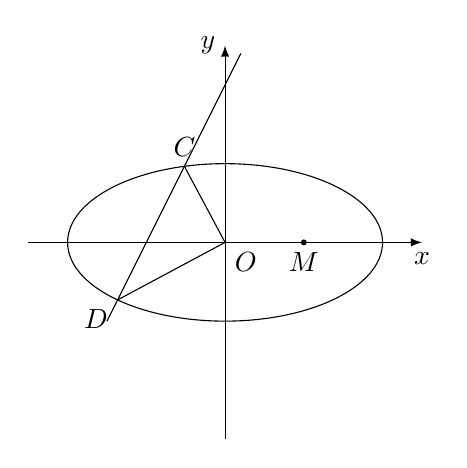
\begin{tikzpicture}[>=latex]
\draw [->] (-2.5,0) -- (2.5,0) node [below] {$x$};
\draw [->] (0,-2.5) -- (0,2.5) node [left] {$y$};
\draw (0,0) node [below right] {$O$};
\draw [name path = elli] (0,0) ellipse (2 and 1);
\draw [domain = -1.5:0.2, name path = line] plot (\x,{2*\x+2});
\draw [name intersections = {of = elli and line, by = {C,D}}];
\draw (0,0) -- (C) node [above] {$C$} (0,0) -- (D) node [below left] {$D$};
\filldraw (1,0) circle (0.03) node [below] {$M$};
\end{tikzpicture}
\end{center}
(1) 求椭圆$\Gamma$的方程;\\
(2) 如图, 过点$P$的直线$l$与椭圆$\Gamma$交于两个不同的点$C$、$D$(点$C$在点$D$的上方), 试求$\triangle COD$面积的最大值;\\
(3) 若直线$m$经过点$M(1, 0)$, 且与椭圆$\Gamma$交于两个不同的点$A$、$B$, 是否存在直线$l_0$: $x=x_0$(其中$x_0>2$), 使得$A$、$B$到直线$l_0$的距离$d_A$、$d_B$满足$\dfrac{d_A}{d_B}=\dfrac{|MA|}{|MB|}$恒成立? 若存在, 求出$x_0$的值; 若不存在, 请说明理由.
\item 给定数列$\{a_n\}$, 若满足$a_1=a$($a>0$且$a\ne 1$), 对于任意的$n, m\in \mathbf{N}^*$, 都有$a_{n+m}=a_n\cdot a_m$, 则称数列$\{a_n\}$为指数数列.\\
(1) 已知数列$\{a_n\}$, $\{b_n\}$的通项公式分别为$a_n=3\cdot 2^{n-1}$, $b_n=3^n$, 试判断$\{a_n\}$, $\{b_n\}$是不是指数数列(需说明理由);\\
(2) 若数列$\{a_n\}$满足: $a_1=2$, $a_2=4$, $a_{n+2}=3a_{n+1}-2a_n$, 证明: $\{a_n\}$是指数数列;\\
(3) 若数列$\{a_n\}$是指数数列, $a_1=\dfrac{t+3}{t+4}$($t\in \mathbf{N}^*$), 证明: 数列$\{a_n\}$中任意三项都不能构成等差数列.

%zmj8
\item 不等式$|1-x|>1$的解集是\blank{50}.
\item 若函数$f(x)=\sqrt {8-ax-2x^2}$是偶函数, 则该函数的定义域是\blank{50}.
\item 若$\sin \alpha =\dfrac 13$, 则$\cos (\alpha -\dfrac{\pi }2)=$\blank{50}.
\item 已知两个不同向量$\overrightarrow{OA}=(1,m)$, $\overrightarrow{OB}=(m-1,2)$, 若$\overrightarrow{OA}\perp \overrightarrow{AB}$, 则实数$m=$\blank{50}.
\item 在等比数列$\{a_n\}$中, 公比$q=2$, 前$n$项和为$S_n$, 若$S_5=1$, 则$S_{10}=$\blank{50}.
\item 若$x$、$y$满足$\begin{cases} x\le 2, \\ x-y+1\ge 0, \\ x+y-2\ge 0, \end{cases}$ 则$z=2x-y$的最小值为\blank{50}.
\item 已知圆$C:(x-4)^2+(y-3)^2=4$和两点$A(-m,0)$, $B(m,0)$, $m>0$, 若圆$C$上至少存在一点$P$, 使得$\angle APB=90^\circ$, 则$m$的取值范围是\blank{50}.
\item $(1+\dfrac 1{x^2})(1+x)^6$展开式中$x^2$项的系数为\blank{50}.
\item 高三某位同学参加物理、化学、政治科目的等级考, 已知这位同学在物理、化学、政治科目考试中达$A^+$的概率分别为$\dfrac 78$、$\dfrac 34$、$\dfrac 5{12}$, 这三门科目考试成绩的结果互不影响, 则这位考生至少得$2$个$A^+$的概率是\blank{50}.
\item 已知$f(x)$是定义在$[-2,2]$上的奇函数, 当$x\in (0,2]$时, $f(x)=2^x-1$, 函数$g(x)=x^2-2x+m$, 如果对于任意的$x_1\in [-2,2]$, 总存在$x_2\in [-2,2]$, 使得$f(x_1)\le g(x_2)$, 则实数$m$的取值范围是\blank{50}.
\item 已知曲线$C:y=-\sqrt {9-x^2}$, 直线$l:y=2$, 若对于点$A(0,m)$, 存在$C$上的点$P$和$l$上的点$Q$, 使得$\overrightarrow{AP}+\overrightarrow{AQ}=\overrightarrow 0$, 则$m$取值范围是\blank{50}.
\item 如图所示, $\angle BAC=\dfrac{2\pi}3$, 圆$M$与$AB$、$AC$分别相切于点$D$、$E$, 点$P$是圆$M$及其内部任意一点, 且$\overrightarrow{AP}=x\overrightarrow{AD}+y\overrightarrow{AE}$($x,y\in \mathbf{R}$), 则$x+y$的取值范围是\blank{50}.
\item 下列函数中, 周期为$\pi$, 且在$[\dfrac{\pi }4,\dfrac{\pi }2]$上为减函数的是\bracket{20}.
\fourch{$y=\sin (2x+\dfrac{\pi }2)$}{$y=\cos (2x+\dfrac{\pi }2)$}{$y=\sin (x+\dfrac{\pi }2)$}{$y=\cos (x+\dfrac{\pi }2)$}
\item 设$\alpha$、$\beta$是两个不同的平面, $b$是直线且$b\subset\beta$, 则``$b\perp \alpha$''是``$\alpha \perp \beta$''的\bracket{20}.
\twoch{充分非必要条件}{必要非充分条件}{充要条件}{既非充分又非必要条件}
\item 若已知极限$\displaystyle\lim_{n\to \infty} \dfrac{\sin n}n=0$, 则$\displaystyle\lim_{n\to \infty} \dfrac{n-3\sin n}{\sin n-2n}$的值为\bracket{20}.
\fourch{$-3$}{$-\dfrac 32$}{$-1$}{$-\dfrac 12$}
\item 若函数$f(x)=\lg [\sin (\pi x)\cdot \sin (2\pi x)\cdot \sin (3\pi x)\cdot \sin (4\pi x)]$的定义域与区间$[0,1]$的交集是$n$个两两不交的开区间的并集, 则$n$的值为\bracket{20}.
\fourch{$2$}{$3$}{$4$}{$5$}
\item 在四棱锥$P-ABCD$中, $PA\perp$平面$ABCD$, $AB\perp AD$, $BC\parallel AD$, $BC=1$, $CD=\sqrt 2$, $\angle CDA=45^{^\circ}$.
\begin{center}
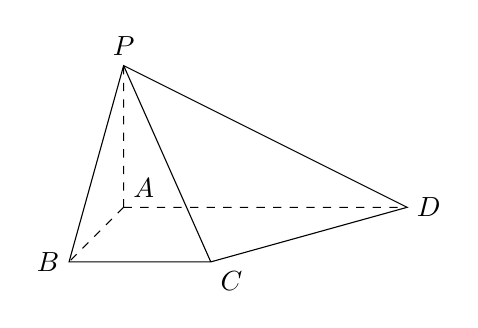
\begin{tikzpicture}[>=latex,scale = 1.8]
\draw (0,0,0) node [above right] {$A$} coordinate (A);
\draw (2,0,0) node [right] {$D$} coordinate (D);
\draw (0,0,1) node [left] {$B$} coordinate (B);
\draw (1,0,1) node [below right] {$C$} coordinate (C);
\draw (0,1,0) node [above] {$P$} coordinate (P);
\draw (P) -- (B) -- (C) -- (D) -- cycle (P) -- (C);
\draw [dashed] (A) -- (B) (A) -- (P) (A) -- (D);
\end{tikzpicture}
\end{center}
(1) 画出四棱锥$P-ABCD$的三视图;\\
(2) 若$PA=BC$, 求直线$PB$与平面$PCD$所成角的大小.
\item 已知椭圆$C:\dfrac{x^2}{a^2}+\dfrac{y^2}{b^2}=1$($a>b>0$)的一个顶点坐标为$A(2,0)$, 且长轴长是短轴长的两倍.\\
(1) 求椭圆$C$的方程;\\
(2) 过点$D(1,0)$且斜率存在的直线交椭圆于$G$、$H$, $G$关于$x$轴的对称点为$G'$, 求证: 直线$G'H$恒过定点$(4,0)$.
\item 某高科技企业研制出一种型号为$A$的精密数控车床, $A$型车床为企业创造的价值逐年减少(以投产一年的年初到下一年的年初为$A$型车床所创造价值的第一年). 若第$1$年$A$型车床创造的价值是$250$万元, 且第$1$年至第$6$年, 每年$A$型车床创造的价值减少$30$万元; 从第$7$年开始, 每年$A$型车床创造的价值是上一年价值的$50\%$. 现用$a_n$($n\in \mathbf{N}^*$)表示$A$型车床在第$n$年创造的价值.\\
(1) 求数列$\{a_n\}$($n\in \mathbf{N}^*$)的通项公式$a_n$;\\
(2) 记$S_n$为数列$\{a_n\}$的前$n$项和, $T_n=\dfrac{S_n}n$. 企业经过成本核算, 若$T_n>100$万元, 则继续使用$A$型车床, 否则在第$n+1$年年初更换$A$型车床. 试问该企业须在第几年年初更换$A$型车床?
\item 设函数$f(x)=|\dfrac 2x-ax+5|$($a\in \mathbf{R}$).\\
(1) 求函数的零点;\\
(2) 当$a=3$时, 求证: $f(x)$在区间$(-\infty ,-1)$上单调递减;\\
(3) 若对任意的正实数$a$, 总存在$x_0\in [1,2]$, 使得$f(x_0)\ge m$, 求实数$m$的取值范围.
\item 给定数列$\{a_n\}$, 若数列$\{a_n\}$中任意(不同)两项之和仍是该数列中的一项, 则称该数列是``封闭数列''.\\
(1) 已知数列$\{a_n\}$的通项公式为$a_n=3^n$, 试判断$\{a_n\}$是否为封闭数列, 并说明理由;\\
(2) 证明: 公差为$d$的等差数列$\{a_n\}$成为``封闭数列''的一个充要条件是: 存在整数$m\ge -1$, 使$a_1=md$;\\
(3) 已知数列$\{a_n\}$满足$a_{n+2}+a_n=2a_{n+1}$且$a_2-a_1=2$, 设$S_n$是该数列$\{a_n\}$的前$n$项和, 试问: 是否存在这样的``封闭数列'' $\{a_n\}$, 使得对任意$n\in \mathbf{N}^*$都有$S_n\ne 0$, 且$\dfrac 18<\dfrac 1{S_1}+\dfrac 1{S_2}+\cdots +\dfrac 1{S_n}<\dfrac{11}{18}$, 若存在, 求数列$\{a_n\}$的首项$a_1$的所有取值, 若不存在, 说明理由.

%zmj9
\item 设$a\in \mathbf{R}$. 已知集合$A=\{a,a^2\}$. 若$1\in A$, 则$a=$\blank{50}.
\item 已知复数$z$满足$z\mathrm{i}=2+\mathrm{i}$($\mathrm{i}$为虚数单位), 则$\mathrm{Im}z=$\blank{50}.
\item 若函数$f(x)=2^x+1$的图像与$y=g(x)$的图像关于直线$y=x$对称, 则$g(3)=$\blank{50}.
\item 若$\tan (\alpha -\dfrac{\pi}4)=-3$, 则$\tan (\pi-\alpha)=$\blank{50}.
\item 如图, 正四棱柱$ABCD-A_1B_1C_1D_1$的底面边长为$3$, 高为$4$, 则异面直线$AA_1$与$BD_1$所成角的大小是\blank{50}.
\begin{center}
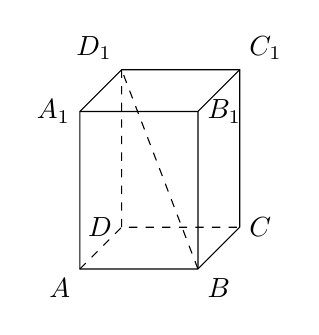
\begin{tikzpicture}[>=latex,scale = 0.5]
\draw (0,0) node [below left] {$A$} coordinate (A) --++ (3,0) node [below right] {$B$} coordinate (B) --++ (45:{3/2}) node [right] {$C$} coordinate (C)
--++ (0,4) node [above right] {$C_1$} coordinate (C1)
--++ (-3,0) node [above left] {$D_1$} coordinate (D1) --++ (225:{3/2}) node [left] {$A_1$} coordinate (A1) -- cycle;
\draw (A) ++ (3,4) node [right] {$B_1$} coordinate (B1) -- (B) (B1) --++ (45:{3/2}) (B1) --++ (-3,0);
\draw [dashed] (A) --++ (45:{3/2}) node [left] {$D$} coordinate (D) --++ (3,0) (D) --++ (0,4);
\draw [dashed] (B) -- (D1);
\end{tikzpicture}
\end{center}
\item 在$(1-2x)^{6}$的二项展开式中, $x^{3}$项的系数为\blank{50}.
\item 新冠病毒爆发初期, 全国支援武汉的活动中, 需要从$A$医院某科室的$7$名男医生(含一名主任医师)、 $5$名女医生(含一名主任医师)中分别选派$3$名男医生和 $2$名女医生, 要求至少有一名主任医师参加, 则不同的选派方案共有\blank{50}种.
\item 设$k\in \{-2,-1,\dfrac 13,\dfrac 23, 2\}$, 若对任意$x\in (-1,0)\cup (0,1)$, 都成立$x^k>\|x|$, 则$k$取值的集合是\blank{50}.
\item 若关于$x,y$的线性方程组$\begin{cases} a_1x+b_1y=c_1, \\ a_2x+b_2y=c_2 \end{cases}$的增广矩阵是$\begin{pmatrix}
m & 1 & 3 \\ 0 & 2 & n  \end{pmatrix}$, 且$\begin{cases} x=-1, \\ y=1 \end{cases}$是该线性方程组的解, 则三阶行列式$\begin{vmatrix}
-1 & 0 & 1  \\ 0 & 3 & m \\ 2 & n & 1  \end{vmatrix}|$中第$3$行第$2$列的元素的代数余子式的值是\blank{50}.
\item 已知定义在$[0,+\infty)$上的函数$f(x)=\begin{cases} 13-|x-1|, & 0\le x<2, \\ f(x-2)-2, & x\ge 2. \end{cases}$设函数$y=f(x)$在$[2n-2,2n)$($n\in \mathbf{N}^*$)上的最大值记作$a_n$. 若用正整数$n$表示$a_n$, 则$a_n=$\blank{50}.
\item 已知平面向量$\overrightarrow a,\overrightarrow b,\overrightarrow c$, 对任意实数t, 都有$|\overrightarrow c-t\overrightarrow a|\ge|\overrightarrow c-\overrightarrow a|$, $|\overrightarrow c-t\overrightarrow b|\ge|\overrightarrow c-\overrightarrow b|$成立. 若$\overrightarrow a\cdot \overrightarrow a=3$, $\overrightarrow b\cdot \overrightarrow b=2$, $\overrightarrow a\cdot \overrightarrow b=1$, 则$|\overrightarrow c|=$\blank{50}.
\item 已知函数$f(x)=|x+\dfrac 1x|$, 给出下列命题:\\
\textcircled{1} 存在实数$a<0$, 函数$y=f(x)+f(x-a)$是偶函数;\\
\textcircled{2} 存在实数$a>0$, 使得函数$y=f(x)+f(x-a)$关于直线$x=1$对称;\\
\textcircled{3} 对于任意实数$a$, 关于$x$的不等式$f(x)+f(x-a)\le 8$总有解.\\
其中的真命题是\blank{50}. (写出所有真命题的序号)
\item 已知$a,b,l$是空间中的三条直线, 其中直线$a,b$在平面$\alpha$上, 则``$l\perp a$且$l\perp b$ ''是``$l\perp$平面$\alpha$''的\bracket{20}条件.
\fourch{充分非必要}{必要非充分}{充要}{既非充分也非必要}
\item 为得到函数$y=\cos x+\sqrt 3\sin x$的图像, 可以将$y=2\cos x$的图像 \bracket{20}个单位.
\fourch{向右平移$\dfrac{\pi}{6}$}{向左平移$\dfrac{\pi}{6}$}{向右平移$\dfrac{\pi}3$}{向左平移$\dfrac{\pi}3$}
\item 某企业欲做一个介绍企业发展史的铭牌, 铭牌的截面形状是如图所示的扇形环面(由扇形$OAD$挖去扇形$OBC$后构成). 已知$OA=10$, $OB=x$($0<x<10$), 线段$BA,CD$、弧$\overset\frown{BC}$、弧$\overset\frown{AD}$的长度之和为$\text{30}$米, 圆心角为$\theta$弧度, 则$\theta =$\bracket{20}.
\begin{center}
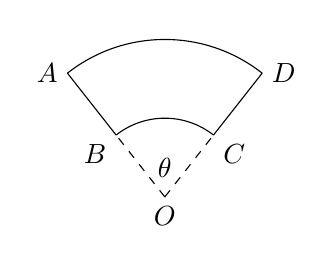
\begin{tikzpicture}[>=latex,scale = 0.2]
\def\t{10/15/pi*180}
\draw (0,0) node [below] {$O$} coordinate (O);
\draw [dashed] (0,0) --++ ({90-\t}:5) node [below right] {$C$} coordinate (C) (0,0) --++ ({90+\t}:5) node [below left] {$B$} coordinate (B);
\draw (B) -- ($(B)!-1!(O)$) node [left] {$A$} coordinate (A) (C) -- ($(C)!-1!(O)$) node [right] {$D$} coordinate (D);
\draw (D) arc ({90-\t}:{90+\t}:10) (C) arc ({90-\t}:{90+\t}:5);
\draw (O) pic ["$\theta$", angle eccentricity = 1.5, scale = 0.5] {angle = C--O--B};
\end{tikzpicture}
\end{center}
\fourch{$\dfrac{10+x}{10+2x}$}{$\dfrac{10+2x}{10+x}$}{$\dfrac{10-x}{10+2x}$}{$\dfrac{10-x}{10+x}$}
\item 在坐标平面内, 点$A$的坐标为$A(5,0)$. 若对于正实数$k$, 总存在函数$f(x)=ax^2$($a>0$), 使$\angle QOA=2\angle POA$, 这里$P(1,f(1))$、$Q(k,f(k))$, 则$k$的取值范围是\bracket{20}.
\fourch{$(2,+\infty)$}{$(3,+\infty)$}{$[4,+\infty)$}{$[8,+\infty)$}
\item 如图, 在圆柱$OO_1$ 中, $AB$是圆柱的母线, $BC$是圆柱的底面$\bigodot O$的直径, $D$是底面圆周上异于$B$、$C$的点.
\begin{center}
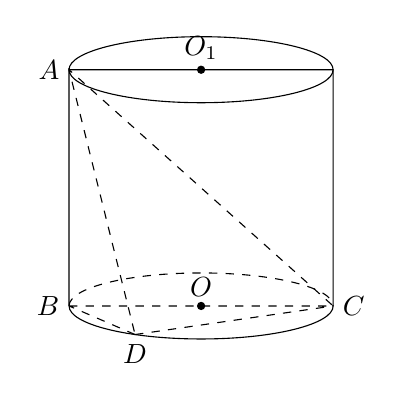
\begin{tikzpicture}[>=latex,scale = 1.5]
\draw ({-sqrt(5)/2},0) node [left] {$B$} coordinate (B) arc (180:360:{sqrt(5)/2} and {sqrt(5)/8}) node [right] {$C$} coordinate (C);
\draw [dashed] ({-sqrt(5)/2},0) arc (180:0:{sqrt(5)/2} and {sqrt(5)/8});
\draw (B) --++ (0,2) node [left] {$A$} coordinate (A) (C) --++ (0,2) -- (A);
\draw (A) arc (180:-180:{sqrt(5)/2} and {sqrt(5)/8});
\filldraw (0,0) circle (0.03) node [above] {$O$} coordinate (O);
\filldraw (O) ++ (0,2) circle (0.03) node [above] {$O_1$} coordinate (O1);
\draw ({sqrt(5)/2*cos(-120)},{sqrt(5)/8*sin(-120)}) node [below] {$D$} coordinate (D);
\draw [dashed] (D) -- (B) (D) -- (C) (B) -- (C) -- (A) -- (D);
\end{tikzpicture}
\end{center}
(1) 求证: $CD\perp AD$.\\
(2) 若$BD=1$, $CD=2$, $AC=3$, 求圆柱$OO_1$的侧面积.
\item 已知函数$f(x)=\sin \dfrac x2\cos \dfrac x2+\cos ^2\dfrac x2-\dfrac 12$.\\
(1) 求函数$y=f(x)$在区间$[0,\pi]$上的值域;\\
(2) 设$\omega >0$. 若关于$x$的方程$4f(\omega x)-\sqrt 2=0$在区间$[0,\pi]$上恰有两个不同的解, 求$\omega$的取值范围.
\item 大数据时代对于数据分析能力的要求越来越高, 数据拟合是一种把现有数据通过数学方法来代入某种算式的表示方式. 比如$A_i(a_i,b_i)$($i=1,2,3,\cdots,n$)是平面直角坐标系上的一系列点, 其中$n$是不小于$2$的正整数, 用函数$y=f(x)$来拟合该组数据, 尽可能使得函数图像与点列$A_i(a_i,b_i)$比较接近. 其中一种衡量接近程度的指标是函数的拟合误差, 拟合误差越小越好, 定义函数$y=f(x)$的拟合误差为:
$$\Delta (f(x))=\dfrac 1n[(f(a_1)-b_1)^2+(f(a_2)-b_2)^2+\cdots +(f(a_n)-b_n)^2].$$
已知在平面直角坐标系上, 有$5$个点的坐标数据如下表所示:
\begin{center}
\begin{tabular}{|c|c|c|c|c|c|}
\hline
$x$ & $1$ & $2$ & $3$ & $4$ & $5$ \\ \hline
$y$ & $2.2$ & $1$ & $2$ & $4.6$ & $7$ \\ \hline
\end{tabular}
\end{center}
(1) 若用函数$f_1(x)=x^2-4x+5$来拟合上述表格中的数据, 求$\Delta (f_1(x))$;\\
(2) 设$m\in \mathbf{R}$. 若用函数$f_2(x)=2^{|x-2|}+m$来拟合上述表格中的数据.\\
\textcircled{1} 求该函数的拟合误差$\Delta (f_2(x))$的最小值, 并求出此时的函数解析式$y=f_2(x)$.\\
\textcircled{2} 根据实数$m$, 讨论用$f_1(x)$, $f_2(x)$(这里$f_2(x)$指\textcircled{1} 中取得$\Delta(f_2(x))$的最小值的那一个)中的哪一个函数来拟合上述表格中的数据更好? 说明理由.
\item 已知椭圆$\Gamma :\dfrac{x^2}6+\dfrac{y^2}2=1$. 直线$l$与$x$轴的正半轴和$y$轴分别交于点$Q,P$, 与椭圆$\Gamma$相交于两点$M\mathbf{N}$, 各点互不重合, 且满足$\overrightarrow{PM}=\lambda_1\overrightarrow{MQ}$, $\overrightarrow{PN}=\lambda_2\overrightarrow{NQ}$.\\
(1) 求焦距, 并证明: 焦距的平方是长轴长的平方、短轴长的平方的等差中项;\\
(2) 若直线$l$的方程为$y=-x+1$, 求$\dfrac 1{\lambda_1}+\dfrac 1{\lambda_2}$的值;\\
(3) 若$\lambda_1+\lambda_2=-3$, 试证明直线$l$恒过定点, 并求此定点的坐标.
\item 已知函数$y=f(x)$的定义域为$\mathbf{R}$, 数列$\{a_n\}$($n\in \mathbf{N}^*$)满足$a_1=1$, $a_2=t$, $a_n=f(a_{n-1})$, $f(a_n)+kf(a_{n-1})=\lambda (a_n+ka_{n-1})$($n\ge 2$, $n\in \mathbf{N}^*)$, 实数$k,t$是非零常数.\\
(1) 若数列$\{a_n\}(n\in \mathbf{N}^{*})$是常数列, 求证: $k=-1$或$\lambda =1$;\\
(2) 若$\lambda =1$, $t<1$, 求证: ``数列$\{a_n\}$($n\in \mathbf{N}^*$)是等差数列''的一个充要条件是``$k=-1$'';\\
(3) 若$k=-1$, $t>1$, 是否存在实数$\lambda$, 使得数列$\{a_n\}$($n\in \mathbf{N}^*$)是等比数列? 若存在, 求$\lambda$的值; 若不存在, 说明理由.

%zmj10
\item 集合$A=\{x|0<x<3\}$, $B=\{x||x|<2\}$, 则$A\cap B=$\blank{50}.
\item 函数$y=x^{-\frac 12}$的定义域是\blank{50}.
\item $\mathrm{i}$是虚数单位, 则$|\dfrac{\mathrm{i}}{1-\mathrm{i}}|$的值为\blank{50}.
\item 已知线性方程组的增广矩阵为$\begin{pmatrix}
1 & 1 & 3  \\ a & 0 & 2  \end{pmatrix}$, 若该线性方程组的解为$\begin{pmatrix}1  \\ 2  \end{pmatrix}$, 则实数$a=$\blank{50}.
\item 已知函数$f(x)=\begin{vmatrix} 2^x & 1  \\ 1 & 1  \end{vmatrix}$, 则$f^{-1}(0)=$\blank{50}.
\item 已知双曲线$\dfrac{x^2}{a^2}-y^2=1(a>0)$的一条渐近线方程为$2x-y=0$, 则实数$a=$\blank{50}.
\item 已知函数$f(x)=\lg \dfrac{1-x}{1+x}+\sin x+1$, 若$f(m)=4$, 则$f(-m)=$\blank{50}.
\item 数列$\{a_n\}$的通项公式$a_n=\begin{cases}
\dfrac 1n, & n=1,2,  \\ \dfrac 1{2^n}, & n\ge 3,  \end{cases}$($n\in \mathbf{N}^*$), 前$n$项和为$S_n$, 则$\displaystyle\lim_{n\to \infty} S_n=$\blank{50}.
\item 甲、乙、丙三个不同单位的医疗队里各有$3$人, 职业分别为医生、护士与化验师, 现在要从中抽取$3$人组建一支志愿者队伍, 则他们的单位与职业都不相同的概率是\blank{50}(结果用最简分数表示).
\item 已知双曲线的中心是坐标原点, 它的一个顶点为$A(\sqrt 2,0)$, 两条渐近线与以$A$为圆心$1$为半径的圆都相切, 则该双曲线的标准方程是\blank{50}.
\item 已知集合$A=\{(x,y)|(x+y)^2+x+y-2\le 0\}$,
$B=\{(x,y)|(x-2a)^2+(y-a-1)^2\le a^2-\dfrac a2\}$, 若$A\cap B\ne \varnothing$, 则实数$a$取值范围为\blank{50}.
\item 设$n\in \mathbf{N}^*$, $a_n$为$(x+2)^n-(x+1)^n$的展开式的各项系数之和, $m=-\dfrac 12t+6$, , $b_n=[\dfrac{a_1}3]+[\dfrac{2a_2}{3^2}]+...+[\dfrac{na_n}{3^n}]$($[x]$表示不超过实数$x$的最大整数), 则当$n$和$t$变动时, $(n-t)^2+(b_n-m)^2$的最小值为\blank{50}.
\item 已知直角坐标平面上两条直线的方程分别为$l_1:a_1x+b_1y+c_1=0$, $l_2:a_2x+b_2y+c_2=0$, 那么``$\begin{vmatrix}
a_1 & b_1  \\a_2 & b_2  \end{vmatrix}=0$''是``两直线$l_1$、$l_2$平行''的\bracket{20}.
\twoch{充分非必要条件}{必要非充分条件}{充要条件}{既非充分又非必要条件}
\item 如图, 若一个水平放置的图形的斜二测直观图是一个底角为$45^\circ$且腰和上底均为$1$的等腰梯形, 则原平面图形的面积是\bracket{20}.
\fourch{$\dfrac{2+\sqrt 2}2$}{$\dfrac{1+\sqrt 2}2$}{$2+\sqrt 2$}{$1+\sqrt 2$}
\item 在正方体$ABCD-A_1B_1C_1D_1$中, 下列结论错误的是\bracket{20}.
\onech{$(\overrightarrow{A_1A}+\overrightarrow{A_1D_1}+\overrightarrow{A_1B_1})^2=3\overrightarrow{A_1B_1}^2$}{$\overrightarrow{A_1C}\cdot (\overrightarrow{A_1B_1}-\overrightarrow{A_1A})=0$}{向量$\overrightarrow{AD_1}$ 与$\overrightarrow{A_1B}$ 的夹角是$120^\circ$}{正方体$ABCD-A_1B_1C_1D_1$的体积为$|\overrightarrow{AB}\cdot \overrightarrow{AA_1}\cdot \overrightarrow{AD}|$}
\item 函数$f(x)$是定义在$\mathbf{R}$上的奇函数, 且$f(x-1)$为偶函数, 当$x\in [0,1]$ 时, $f(x)=\sqrt x$.若函数$g(x)=f(x)-x-m$ 有三个零点, 则实数$m$的取值范围是\bracket{20}.
\twoch{$(-\dfrac 14,\dfrac 14)$}{$(1-\sqrt {2},\sqrt {2}-1)$}{$\{m|4k-\dfrac 14<m<4k+\dfrac 14,k\in \mathbf{Z}\}$}{$\{m|4k+1-\sqrt 2<m<4k+\sqrt 2-1,k\in \mathbf{Z}\}$}
\item 如图, 已知四棱锥$P-ABCD,PA\perp$底面$ABCD$, $PA=1$, 底面$ABCD$是正方形, $E$是$PD$的中点, $PD$与底面$ABCD$所成角的大小为$\dfrac{\pi }6$.
\begin{center}
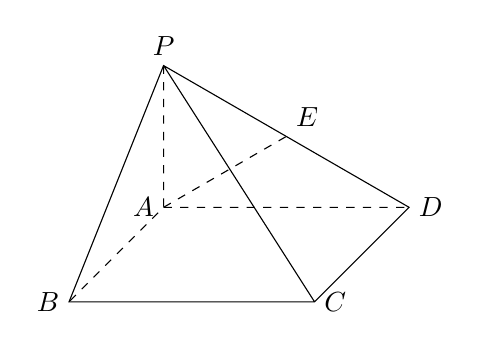
\begin{tikzpicture}[>=latex, scale = 1.8]
\draw (0,0,0) node [left] {$A$} coordinate (A);
\draw ({sqrt(3)},0,0) node [right] {$D$} coordinate (D);
\draw (0,0,{sqrt(3)}) node [left] {$B$} coordinate (B);
\draw ({sqrt(3)},0,{sqrt(3)}) node [right] {$C$} coordinate (C);
\draw (0,1,0) node [above] {$P$} coordinate (P);
\draw (P) -- (B) -- (C) -- (D) -- cycle (P) -- (C);
\draw [dashed] (P) -- (A) -- (B) (A) -- (D);
\draw ($(P)!0.5!(D)$) node [above right] {$E$} coordinate (E);
\draw [dashed] (A) -- (E);
\end{tikzpicture}
\end{center}
(1) 求四棱锥$P-ABCD$的体积;\\
(2) 求异面直线$AE$与$PC$所成角的大小.
\item 已知函数$f(x)=2\cos ^2\dfrac x2+\sqrt 3\sin x$.\\
(1) 求函数$f(x)$在区间$[0,\pi]$上的单调递增区间;\\
(2) 当$f(\alpha)=\dfrac{11}{5}$, 且$-\dfrac{2\pi}3<\alpha <\dfrac{\pi}6$, 求$\sin (2\alpha +\dfrac{\pi}3)$的值.
\item 随着疫情的有效控制, 人们的生产生活逐渐向正常秩序恢复, 位于我区的某著名赏花园区重新开放.据统计研究, 近期每天赏花的人数大致符合以下数学模型($n\in \mathbf{N}^*$):\\
以$f(n)=\begin{cases}
200n+1500, & 1\le n\le 6,  \\ 300\cdot 3^{\frac{n-6}{11}}+2400, & 7\le n\le 28,  \\ 23400-650n, & 29\le n\le 36 \end{cases}$表示第$n$个时刻进入园区的人数;\\
以$g(n)=\begin{cases}
0, & 1\le n\le 15,  \\ 400n-5000, & 16\le n\le 28,  \\ 8200, & 29\le n\le 36  \end{cases}$表示第$n$个时刻离开园区的人数.\\
设定每$15$分钟为一个计算单位, 上午$8$点$15$分作为第$1$个计算人数单位, 即$n=1$; $8$点$30$分作为第$2$个计算单位, 即$n=2$; 依次类推, 把一天内从上午$8$点到下午$5$点分成$36$个计算单位(最后结果四舍五入, 精确到整数).\\
(1) 试分别计算当天$12: 30$至$13: 30$这一小时内, 进入园区的游客人数$f(19)+f(20)+f(21)+f(22)$和离开园区的游客人数$g(19)+g(20)+g(21)+g(22)$;\\
(2) 请问, 从$12$点(即$n=16$)开始, 园区内游客总人数何时达到最多? 并说明理由.
\item 已知动直线$l$与椭圆C:$x^2+\dfrac{y^2}2=1$交于$P(x_1,y_1)$、$Q(x_2,y_2)$两不同点, 且$\triangle OPQ$的面积$S_{\triangle OPQ}=\dfrac{\sqrt 2}2$, 其中$O$为坐标原点.\\
(1) 若动直线$l$垂直于$x$轴, 求直线$l$的方程;\\
(2) 证明$x_1^2+x_2^2$和$y_1^2+y_2^2$均为定值;\\
(3) 椭圆$C$上是否存在点$D,E,G$, 使得三角形面积$S_{\triangle ODE}=S_{\triangle ODG}=S_{\triangle OEG}=\dfrac{\sqrt 2}2$? 若存在, 判断$\triangle DEG$的形状; 若不存在, 请说明理由.
\item 若无穷数列$\{a_n\}$满足: 存在$k,n_0\in \mathbf{N}^*$, 对任意的$n\ge n_0$($n\in \mathbf{N}^*$), 都有$a_{n+k}-a_n=d$($d$为常数), 则称 $\{a_n\}$具有性质$Q(k,n_0,d)$.\\
(1) 若无穷数列$\{a_n\}$具有性质$Q(3,1,0)$, 且$a_1=1$, $a_2=2$, $a_3=3$, 求$a_2+a_3+a_4$的值;\\
(2) 若无穷数列$\{b_n\}$是等差数列, 无穷数列$\{c_n\}$是公比为正数的等比数列, $b_1=c_5=1$, $b_5=c_1=81$, $a_n=b_n+c_n$, 判断$\{a_n\}$是否具有性质$Q(k,n_0,0)$, 并说明理由;\\
(3) 设无穷数列$\{a_n\}$既具有性质$Q(i,2,d_1)$, 又具有性质$Q(j,2,d_2)$, 其中$i,j\in \mathbf{N}^*$, $i<j$, $i$和$j$互质, 求证: 数列$\{a_n\}$具有性质$Q(j-i,2,\dfrac{j-i}id_1)$.

%zmj11
\item $\displaystyle\lim_{n\to \infty}\dfrac{3^n}{3^n+2^n}=$\blank{50}.
\item 若集合$A=\{x|-1<x<3\}$, $B=\{1,2,3,4\}$, 则$A\cap B=$\blank{50}.
\item 已知复数$z$满足$z\cdot (1-\mathrm{i})=1+\mathrm{i}$($\mathrm{i}$为虚数单位), 则$|z|=$\blank{50}.
\item 若$\sin \alpha =\dfrac 13$, 则$\cos (\pi -2\alpha)=$\blank{50}.
\item 抛物线$y^2=-4x$的准线方程是\blank{50}.
\item 已知函数$y=f(x)$的图像与函数$y=2^x$的图像关于$y=x$对称, 则$f(3)=$\blank{50}.
\item 从包含学生甲的$1200$名学生中随机抽取一个容量为$80$的样本, 则学生甲被抽到的概率为\blank{50}.
\item 在$(x^2+\dfrac 2x)^6$的二项展开式中, 常数项等于\blank{50}.
\item 在$\triangle ABC$中, 角$A$、$B$、$C$所对的边分别为$a$、$b$、$c$, 且$\begin{vmatrix}
\sqrt 3b+2c & 2a  \\\cos B & 1  \end{vmatrix}=0$, 则角$A=$\blank{50}.
\item 从以下七个函数:
$y=x$, $y=\dfrac 1x$, $y=x^2$, $y=2^x$, $y=\log_2x$, $y=\sin x$, $y=\cos x$中选取两个函数记为$f(x)$和$g(x)$, 构成函数$F(x)=f(x)+g(x)$, 若$F(x)$的图像如图所示, 则$F(x)=$\blank{50}.
\begin{center}
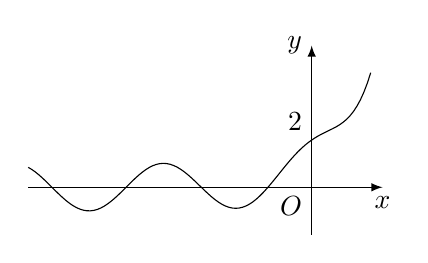
\begin{tikzpicture}[>=latex, scale = 0.3]
\draw [->] (-12,0) -- (3,0) node [below] {$x$};
\draw [->] (0,-2) -- (0,6) node [left] {$y$};
\draw (0,0) node [below left] {$O$};
\draw [domain = -12:2.5, samples = 100] plot (\x,{pow(2,\x)+cos(\x/pi*180)});
\draw (0,2) node [above left] {$2$};
\end{tikzpicture}
\end{center}
\item 已知平面向量$\overrightarrow a,\overrightarrow b,\overrightarrow c$满足$|\overrightarrow a|=|\overrightarrow b|=|\overrightarrow c|=1$, 且$\overrightarrow a\cdot \overrightarrow b=\dfrac 12$, 若存在实数$x,y$, 使得$\overrightarrow c=x\overrightarrow a+y\overrightarrow b$, 则$x+y$的最大值为\blank{50}.
\item 已知函数$f(x)=\begin{cases}|5^x-1|, & x<1, \\ \dfrac{8}{x+1},& x\ge 1,  \end{cases}$, 若方程$f(f(x))=a$恰有$5$个不同的实数根, 则实数$a$的取值范围为\blank{50}.
\item 已知两条直线$l_1$、$l_2$的方程分别为$l_1:ax+y-1=0$和$l_2:x-2y+1=0$, 则``$a=2$''是``直线$l_1\perp l_2$''的\bracket{20}.
\twoch{充分不必要条件}{必要不充分条件}{充要条件}{既不充分也不必要条件}
\item 在正方体$ABCD-A_1B_1C_1D_1$ 中, 下列四个结论中错误的是\bracket{20}.
\begin{center}
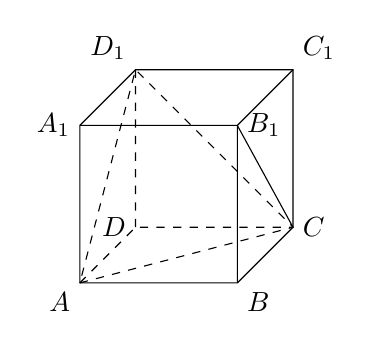
\begin{tikzpicture}[>=latex]
\draw (0,0) node [below left] {$A$} coordinate (A) --++ (2,0) node [below right] {$B$} coordinate (B) --++ (45:{2/2}) node [right] {$C$} coordinate (C)
--++ (0,2) node [above right] {$C_1$} coordinate (C1)
--++ (-2,0) node [above left] {$D_1$} coordinate (D1) --++ (225:{2/2}) node [left] {$A_1$} coordinate (A1) -- cycle;
\draw (A) ++ (2,2) node [right] {$B_1$} coordinate (B1) -- (B) (B1) --++ (45:{2/2}) (B1) --++ (-2,0);
\draw [dashed] (A) --++ (45:{2/2}) node [left] {$D$} coordinate (D) --++ (2,0) (D) --++ (0,2);
\draw (B1) -- (C);
\draw [dashed] (A) -- (C) -- (D1) -- cycle;
\end{tikzpicture}
\end{center}
\onech{直线$B_1C$与直线$AC$所成的角为$60^\circ$}{直线$B_1C$与平面$AD_1C$所成的角为$60^\circ$}{直线$B_1C$与直线$AD_1$所成的角为$90^\circ$}{直线$B_1C$与直线$AB$所成的角为$90^\circ$}
\item 已知实数$x>0$, $y>0$, 且$2x+\dfrac 1y=1$, 则$\dfrac yx$的\bracket{20}.
\fourch{最小值为$8$}{最大值为$8$}{最小值为$2$}{最大值为$2$}
\item 在平面上, 已知定点$A(2,0)$, 动点$P(\sin\alpha,\cos\alpha)$. 当$\alpha$在区间$[-\dfrac \pi 4,\dfrac \pi 4]$上变化时, 动线段$AP$所形成图形的面积为\bracket{20}.
\fourch{$\sqrt 2-\dfrac \pi 4$}{$\sqrt 3-\dfrac\pi 4$}{$\dfrac{5\pi}{24}+\dfrac{\sqrt 3}2-\dfrac{\sqrt 2}2$}{$\dfrac \pi 4$}
\item 如图1, 在三棱柱$ABC-A_1B_1C_1$中, 已知$AB\perp AC$, $AB=AC=1$, $AA_1=2$, 且$AA_1\perp$平面$ABC$. 过$A_1$、$C_1$、$B$三点作平面截此三棱柱, 截得一个三棱锥和一个四棱锥(如图2).
\begin{center}
\begin{tikzpicture}[>=latex]
\draw (0,0,0) node [left] {$A$} coordinate (A);
\draw (1,0,0) node [right] {$B$} coordinate (B);
\draw (0,0,1) node [left] {$C$} coordinate (C);
\draw (A) ++ (0,2,0) node [above] {$A_1$} coordinate (A1);
\draw (B) ++ (0,2,0) node [right] {$B_1$} coordinate (B1);
\draw (C) ++ (0,2,0) node [left] {$C_1$} coordinate (C1);
\draw (A1) -- (B1) -- (B) -- (C) -- (C1) -- cycle (C1) -- (B1) (C1) -- (B);
\draw [dashed] (A) -- (C) (A) -- (B) (A) -- (A1) (A1) -- (B);
\draw (0.5,-0.8) node {图1};
\draw (A) ++ (3,0) node [left] {$A$} coordinate (A3);
\draw (B) ++ (3,0) node [right] {$B$} coordinate (B3);
\draw (C) ++ (3,0) node [left] {$C$} coordinate (C3);
\draw (C3) ++ (0,2) node [left] {$C_1$} coordinate (C4);
\draw (A3) ++ (0,2) node [above] {$A_1$} coordinate (A4);
\draw (B3) -- (C3) -- (C4) -- (A4) -- cycle (B3) -- (C4);
\draw [dashed] (A3) -- (B3) (A3) -- (C3) (A3) -- (A4);
\draw (B) ++ (4.5,0) node [right] {$B$} coordinate (B5);
\draw (B5) ++ (0,2) node [right] {$B_1$} coordinate (B6);
\draw (C1) ++ (4.5,0) node [left] {$C_1$} coordinate (C6);
\draw (A1) ++ (4.5,0) node [above] {$A_1$} coordinate (A6);
\draw (C6) -- (B5) -- (B6) -- (A6) -- cycle (B6) -- (C6);
\draw [dashed] (A6) -- (B5);
\draw (4.25,-0.8) node {图2};
\end{tikzpicture}
\end{center}
(1) 求异面直线$BC_1$与$AA_1$所成角的大小(结果用反三角函数表示);\\
(2) 求四棱锥$B-ACC_1A_1$的体积和表面积.
\item 已知函数$f(x)=\sqrt 3\sin x\cos x+\cos ^2x+1$.\\
(1) 求$f(x)$的最小正周期和值域;\\
(2) 若对任意的$x\in \mathbf{R}$, $f^2(x)-k\cdot f(x)-2\le 0$恒成立, 求实数$k$的取值范围.
\item 某网店有$3$(万件)商品, 计划在元旦旺季售出商品$x$(万件). 经市场调查测算, 花费$t$(万元)进行促销后, 商品的剩余量$3-x$与促销费$t$之间的关系为$3-x=\dfrac k{t+1}$(其中$k$为常数), 如果不搞促销活动, 只能售出$1$(万件)商品.\\
(1) 要使促销后商品的剩余量不大于$0.1$(万件), 促销费$t$至少为多少(万元)?\\
(2) 已知商品的进价为$32$(元/件), 另有固定成本$3$(万元). 定义每件售出商品的平均成本为$32+\dfrac 3x$(元).若将商品售价定为: ``每件售出商品平均成本的$1.5$倍''与``每件售出商品平均促销费的一半''之和, 则当促销费$t$为多少(万元)时, 该网店售出商品的总利润最大? 此时商品的剩余量为多少?
\item 已知椭圆$\Gamma \dfrac{x^2}{a^2}+\dfrac{y^2}{b^2}=1$($a>b>0$)的右焦点坐标为$(2,0)$, 且长轴长为短轴长的$\sqrt 2$倍. 直线$l$交椭圆$\Gamma$于不同的两点$M$和$N$.
\begin{center}
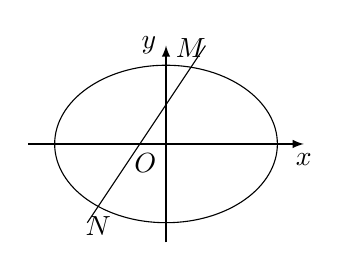
\begin{tikzpicture}[>=latex, scale = 0.5]
\draw [->] (-3.5,0) -- (3.5,0) node [below] {$x$};
\draw [->] (0,-2.5) -- (0,2.5) node [left] {$y$};
\draw (0,0) node [below left] {$O$};
\draw [name path = elli] (0,0) ellipse ({sqrt(8)} and 2);
\draw [name path = line] (1,2.5) -- (-2,-2);
\draw [name intersections = {of = elli and line, by = {M,N}}];
\draw (M) node [above] {$M$};
\draw (N) node [below] {$N$};
\end{tikzpicture}
\end{center}
(1) 求椭圆$\Gamma$的方程;\\
(2) 若直线$l$经过点$T(0,4)$, 且$\triangle OMN$的面积为$2\sqrt 2$, 求直线$l$的方程;\\
(3) 若直线$l$的方程为$y=kx+t$($k\ne 0$), 点$M$关于$x$轴的对称点为$M'$, 直线$MN$、$M'N$ 分别与$x$轴相交于$P$、$Q$两点, 求证: $|OP|\cdot|OQ|$为定值.
\item 对于由$m$个正整数构成的有限集$M=\{a_1,a_2,a_3,\cdots ,a_m\}$, 记$P(M)=a_1+a_2+\cdots +a_m$, 特别规定$P(\varnothing)=0$. 若集合$M$满足: 对任意的正整数$k\le P(M)$, 都存在集合$M$的两个子集$A$、$B$, 使得$k=P(A)-P(B)$成立, 则称集合$M$为``满集''.\\
(1) 分别判断集合$M_1=\{1,2\}$与$M_2=\{1,4\}$是否是``满集'', 请说明理由;\\
(2) 若$a_1,a_2,\cdots ,a_m$是公差为$d(d\in \mathbf{N}^*)$的等差数列, 求证: 集合$M$为``满集''的必要条件是$a_1=1$, $d=1$或$2$;\\
(3) 若$a_1,a_2,\cdots ,a_m$由小到大能排列成首项为$1$, 公比为$3$的等比数列, 求证: 集合$M$是``满集''.

%zmj12
\item 设全集$U=\mathbf{R}$, 若集合$A=\{1,2,3,4\}$, $B=\{x|2\le x\le 3\}$, 则$A\cap \complement _UB\text=$\blank{50}.
\item 已知点$(2,5)$在函数$f(x)=1+a^x$($a>0$且$a\ne 1$)的图像上, 则$f(x)$的反函数$f^{-1}(x)=$\blank{50}.
\item 不等式$\dfrac{x+1}x>1$的解为\blank{50}.
\item 已知球的主视图所表示图形的面积为$9\pi$, 则该球的体积是\blank{50}.
\item 函数$f(x)=\begin{vmatrix}
\cos 2x & -\sin x  \\\cos x & \dfrac{\sqrt 3}2  \end{vmatrix}$在区间$[0,\dfrac{\pi}{2}]$上的最小值为\blank{50}.
\item 若$2+\mathrm{i}$($\mathrm{i}$是虚数单位)是关于$x$的实系数方程$x^2+mx+n=0$的一个根, 则圆锥曲线$\dfrac{x^2}m+\dfrac{y^2}n=1$的焦距为\blank{50}.
\item 已知点$O(0,0)$, $A(2,0)$, $B(1,-2\sqrt 3)$, $P$是曲线$y=\sqrt {1-\dfrac{x^2}4}$上一个动点, 则$\overrightarrow{OP}\cdot \overrightarrow{BA}$的取值范围是\blank{50}.
\item 甲、乙两队进行排球决赛, 现在的情形是甲队只要再赢一局就获冠军, 乙队需要再赢两局才能得冠军.若两队在每局赢的概率都是$0.5$, 则甲队获得冠军的概率为\blank{50}.(结果用数值表示)
\item 已知函数$f(x)=x+\dfrac 4x-1$, 若存在$x_1,x_2,\cdots ,x_n\in [\dfrac 14,4]$使得$f(x_1)+f(x_2)+\cdots +f(x_{n-1})=f(x_n)$, 则正整数$n$的最大值是\blank{50}.
\item 在平面直角坐标系中, 设点$O(0,0)$, $A(3,\sqrt 3)$, 点$P(x,y)$的坐标满足$\begin{cases} \sqrt 3x-y\le 0, \\ x-\sqrt 3y+2\ge 0, \\ y\ge 0 ,\end{cases}$则$\overrightarrow{OA}$在$\overrightarrow{OP}$上的投影的取值范围是\blank{50}.
\item 函数$f(x)=\sin \omega x$($\omega >0$)的图像与其对称轴在$y$轴右侧的交点从左到右依次记为$A_1,A_2,A_3,\cdots ,A_n,\cdots$, 在点列$\{A_n\}$中存在三个不同的点$A_k$、$A_i$、$A_p$, 使得$\triangle A_kA_iA_p$是等腰直角三角形, 将满足上述条件的$\omega$值从小到大组成的数列记为$\{\omega _n\}$, 则$\omega_{2019}=$\blank{50}.
\item 我们把一系列向量$\overrightarrow{a_i}$($i=1,2,\cdots ,n)$按次序排成一列, 称为向量列, 记作$\{\overrightarrow{a_i}\}$, 已知向量列$\{\overrightarrow{a_i}\}$满足$\overrightarrow{a_1}=(1,1)$, $\overrightarrow{a_n}=(x_n,y_n)=\dfrac 12(x_{n-1}-y_{n-1},x_{n-1}+y_{n-1})$($n\ge 2$), 设$\theta_n$表示向量$\overrightarrow{a_{n-1}}$与$\overrightarrow{a_n}$的夹角, 若$b_n=\dfrac{n^2}{\pi}\theta_n$, 对任意正整数$n$, 不等式$\sqrt{\dfrac 1{b_{n+1}}}+\sqrt {\dfrac 1{b_{n+2}}}+\cdots +\sqrt {\dfrac 1{b_{2n}}}>\log_a(1-2a)$恒成立, 则实数$a$的取值范围是\blank{50}.
\item 满足条件$|z-\mathrm{i}|=|3+4\mathrm{i}|$($\mathrm{i}$是虚数单位)的复数$z$在复平面上对应的点的轨迹是\bracket{20}.
\fourch{直线}{圆}{椭圆}{双曲线}
\item 设$n\in \mathbf{N}^*$, 则``数列$\{a_n\}$为等比数列''是``数列$\{a_n\}$满足$a_n\cdot a_{n+3}=a_{n+1}\cdot a_{n+2}$''的\bracket{20}.
\twoch{充分非必要条件}{必要非充分条件}{充要条件}{既非充分也非必要条件}
\item 已知直线$l_1:4x-3y+6=0$和直线$l_2:x=-1$, 则抛物线$y^2=4x$上一动点$P$到直线$l_1$和直线$l_2$的距离之和的最小值是\bracket{20}.
\fourch{$\dfrac{37}{16}$}{$\dfrac{11}{5}$}{$2$}{$\dfrac{7}{4}$}
\item 已知$\{a_n\}$是公差为$d$($d>0$)的等差数列, 若存在实数$x_1, x_2, x_3, \cdots, x_9$满足方程组$$\begin{cases} \sin x_1+\sin x_2+\sin x_3+\cdots +\sin x_9=0, \\ a_1\sin x_1+a_2\sin x_2+a_3\sin x_3+\cdots +a_9\sin x_9=25, \end{cases}$$则$d$的最小值为\bracket{20}.
\fourch{$\dfrac 98$}{$\dfrac 89$}{$\dfrac 54$}{$\dfrac 45$}
\item 在$\triangle ABC$中, 角$A$, $B$, $C$的对边分别是$a$, $b$, $c$, 且$2\cos 2A+4\cos (B+C)+3=0$.\\
(1) 求角$A$的大小;\\
(2) 若$a=\sqrt 3$, $b+c=3$, 求$b$和$c$的值.
\item 如图: 正四棱柱$ABCD-A_1B_1C_1D_1$中, 底面边长为$2$, $BC_1$与底面$ABCD$所成角的大小为$\arctan 2$, $M$是$DD_1$的中点, $N$是$BD$上的一动点, 设$\overrightarrow{DN}=\lambda \overrightarrow{DB}(0<\lambda <1)$.
\begin{center}
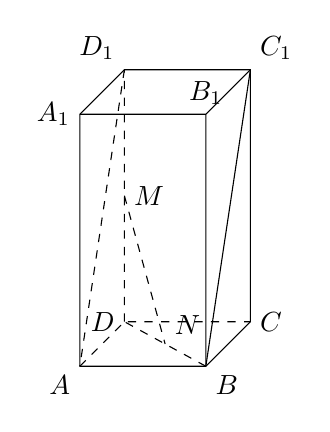
\begin{tikzpicture}[>=latex,scale = 0.8]
\draw (0,0) node [below left] {$A$} coordinate (A) --++ (2,0) node [below right] {$B$} coordinate (B) --++ (45:{2/2}) node [right] {$C$} coordinate (C)
--++ (0,4) node [above right] {$C_1$} coordinate (C1)
--++ (-2,0) node [above left] {$D_1$} coordinate (D1) --++ (225:{2/2}) node [left] {$A_1$} coordinate (A1) -- cycle;
\draw (A) ++ (2,4) node [above] {$B_1$} coordinate (B1) -- (B) (B1) --++ (45:{2/2}) (B1) --++ (-2,0);
\draw [dashed] (A) --++ (45:{2/2}) node [left] {$D$} coordinate (D) --++ (2,0) (D) --++ (0,4);
\draw ($(D)!0.5!(D1)$) node [right] {$M$} coordinate (M);
\draw ($(D)!0.5!(B)$) node [above right] {$N$} coordinate (N);
\draw [dashed] (B) -- (D) (M) -- (N) (D1) -- (A);
\draw (B) -- (C1);
\end{tikzpicture}
\end{center}
(1) 当$\lambda =\dfrac{1}{2}$时, 证明: $MN$与平面$ABC_1D_1$平行;\\
(2) 若点$N$到平面$BCM$的距离为$d$, 试用$\lambda$表示$d$, 并求出$d$的取值范围.
\item $2018$年世界人工智能大会已于$2018$年$9$月在上海徐汇西岸举行, 某高校的志愿者服务小组受大会展示项目的启发, 会后决定开发一款``猫捉老鼠''的游戏.如下图: $A$、$B$两个信号源相距$10$米, $O$是$AB$的中点, 过$O$点的直线$l$与直线$AB$的夹角为$45^\circ$.机器猫在直线$l$上运动, 机器鼠的运动轨迹始终满足: 接收到$A$点的信号比接收到$B$点的信号晚$\dfrac 8{v_0}$秒(注: 信号每秒传播$v_0$米).在时刻$t_0$时, 测得机器鼠距离$O$点为$4$米.
\begin{center}
\begin{tikzpicture}[>=latex]
\draw [->] (-2,0) -- (2,0) node [below] {$x$};
\draw [->] (0,-2) -- (0,2) node [left] {$y$};
\draw (0,0) node [below right] {$O$};
\filldraw (-1,0) circle (0.03) node [below] {$A$} coordinate (A);
\filldraw (1,0) circle (0.03) node [below] {$B$} coordinate (B);
\draw (-1.6,-1.6) -- (1.6,1.6) node [right] {$l$};
\draw (0.8,0.8) node [fill = white] {\rotatebox{45}{猫}};
\draw ({4/3},0.8) node {鼠};
\end{tikzpicture}
\end{center}
(1) 以$O$为原点, 直线$AB$为$x$轴建立平面直角坐标系(如图), 求时刻$t_0$时机器鼠所在位置的坐标;\\
(2) 游戏设定: 机器鼠在距离直线$l$不超过$1.5$米的区域运动时, 有``被抓''的风险.如果机器鼠保持目前的运动轨迹不变, 是否有``被抓''风险?
\item 对于项数为$m(m\ge 3)$的有穷数列$\{a_n\}$, 若存在项数为$m+1$, 公差为$d$的等差数列$\{b_n\}$, 使得$b_k<a_k<b_{k+1}$, 其中$k=1,2,\ldots ,m$, 则称数列$\{a_n\}$为``等差分割数列''.\\
(1) 判断数列$\{a_n\}:1,4,8,13$是否为``等差分割数列'', 并说明理由;\\
(2) 若数列$\{a_n\}$的通项公式为$a_n=2^n$($n=1,2,\cdots ,m$), 求证: 当$m\ge 5$时, 数列$\{a_n\}$不是``等差分割数列'';\\
(3) 已知数列$\{a_n\}$的通项公式为$a_n=4n+3$($n=1,2,\cdots ,m$), 且数列$\{a_n\}$为``等差分割数列''.若数列$\{b_n\}$的首项$b_1=3$, 求数列$\{b_n\}$的公差$d$的取值范围(用$m$表示).
\item 已知函数$y=f_1(x)$, $y=f_2(x)$, 定义函数$f(x)=\begin{cases} f_1(x), & f_1(x)\le f_2(x), \\ f_2(x), & f_1(x)>f_2(x). \end{cases}$\\
(1) 设函数$f_1(x)=\sqrt x$, $f_2(x)=(\dfrac 12)^{x-1}$($x\ge 0$), 求函数$y=f(x)$的值域;\\
(2) 设函数$f_1(x)=\lg (|p-x|+1)$($0<x\le \dfrac 12$, $p$为实常数), $f_2(x)=\lg \dfrac 1x$($0<x\le \dfrac 12$), 当$0<x\le \dfrac 12$时, 恒有$f(x)=f_1(x)$, 求实常数$p$的取值范围;\\
(3) 设函数$f_1(x)=2^{|x|}$, $f_2(x)=3\cdot 2^{|x-p|}$, $p$为正常数, 若关于$x$的方程$f(x)=m$($m$为实常数)恰有三个不同的解, 求$p$的取值范围及这三个解的和(用$p$表示).

%zmj12
\item 若集合$A=(-\infty ,-3)$, $B=(-4,+\infty)$, 则$A\cap B=$\blank{50}.
\item 抛物线$y^2=6x$的准线方程为\blank{50}.
\item 已知复数$z$满足$\dfrac 1{z-1}=\mathrm{i}$($\mathrm{i}$为虚数单位), 则$z=$\blank{50}.
\item 设向量$\overrightarrow a = (1,2)$, $\overrightarrow b = (2,1)$, 则$\overrightarrow a$与$\overrightarrow b$的夹角的大小为\blank{50}(结果用反三角函数值表示).
\item 已知二项式$(2x+\dfrac 1x)^6$, 则其展开式中的常数项为\blank{50}.
\item 若实数$x,y$满足$\begin{cases} x\ge 0, \\ 2x-y \le 0, x+y-3\le 0,\end{cases}$则$z=2x+y$的最大值为\blank{50}.
\item 已知圆锥的底面半径为$1$, 高为$\sqrt 3$, 则该圆锥的侧面展开图的圆心角$\theta$的大小为\blank{50}.
\item 方程$\cos 2x-\sin x=0$在区间$[0,\pi]$上的所有解的和为\blank{50}.
\item 已知函数$f(x)$的周期为$2$, 且当$0<x\le 1$时, $f(x)=\log_4x$, 那么$f(\dfrac 92)=$\blank{50}.
\item 设数列$\{x_n\}$的前$n$项和为$S_n$, 对任意$n\in \mathbf{N}^*$, 均有$S_n+x_n=-1$, 则$S_6=$\blank{50}.
\item 对于函数$f(x)=\sqrt {ax^2+bx}$, 其中$b>0$, 若$f(x)$的定义域与值域相同, 则非零实数$a$的值为\blank{50}.
\item 已知函数$f(x)=\begin{cases}  -2x, & x<0, \\  x^2-1, & x\ge 0,\end{cases}$若方程$f(x)+2\sqrt {1-x^2}+|f(x)-2\sqrt {1-x^2}|-2ax-4=0$有三个根$x_1<x_2<x_3$, 且$x_3-x_2=2(x_2-x_1)$, 则实数$a=$\blank{50}.
\item 直线$x+3y-1=0$的一个法向量可以是\bracket{20}.
\fourch{$(3,-1)$}{$(3,1)$}{$(1,3)$}{$(-1,3)$}
\item ``函数$f(x)=\sin (\omega x)$($x,\omega \in \mathbf{R}$, 且$\omega \ne 0$)的最小正周期为$2$''是``$\omega =\pi$''的\bracket{20}.
\twoch{充分非必要条件}{必要非充分条件}{充要条件}{既非充分又非必要条件}
\item 从$0,1,2,3,4,5,6,7,8,9$这$10$个数中任取$5$个不同的数, 则这$5$个不同的数的中位数为$4$的概率为\bracket{20}.
\fourch{$\dfrac 1{21}$}{$\dfrac 3{21}$}{$\dfrac 5{21}$}{$\dfrac 7{21}$}
\item 下列结论中错误的是\bracket{20}.
\onech{存在实数$x$、$y$满足$\begin{cases}|x|\le 1, \\|x+y|\le 1, \end{cases}$ 并使得$4(x+1)(y+1)>9$成立}{存在实数$x$、$y$满足$\begin{cases}|x|\le 1, \\|x+y|\le 1, \end{cases}$ 并使得$4(x+1)(y+1)>7$成立}{满足$\begin{cases}|x|\le 1, \\|x+y|\le 1, \end{cases}$ 且使得$4(x+1)(y+1)=-9$的实数$x$、$y$不存在}{满足$\begin{cases}|x|\le 1, \\|x+y|\le 1, \end{cases}$ 且使得$4(x+1)(y+1)<-9$的实数$x$、$y$不存在}
\item 如图, 在长方体$ABCD=A_1B_1C_1D_1$中, $T$为$DD_1$上一点, 已知$DT=2$, $AB=4$, $BC=2$, $AA_1=6$.
\begin{center}
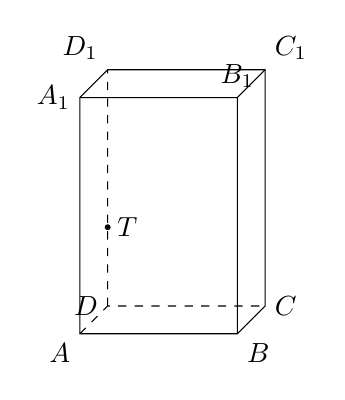
\begin{tikzpicture}[>=latex, scale = 0.5]
\draw (0,0) node [below left] {$A$} coordinate (A) --++ (4,0) node [below right] {$B$} coordinate (B) --++ (45:{2/2}) node [right] {$C$} coordinate (C)
--++ (0,6) node [above right] {$C_1$} coordinate (C1)
--++ (-4,0) node [above left] {$D_1$} coordinate (D1) --++ (225:{2/2}) node [left] {$A_1$} coordinate (A1) -- cycle;
\draw (A) ++ (4,6) node [above] {$B_1$} coordinate (B1) -- (B) (B1) --++ (45:{2/2}) (B1) --++ (-4,0);
\draw [dashed] (A) --++ (45:{2/2}) node [left] {$D$} coordinate (D) --++ (4,0) (D) --++ (0,6);
\filldraw ($(D)!{1/3}!(D1)$) circle (0.06) node [right] {$T$};
\end{tikzpicture}
\end{center}
(1) 求直线$TC$与平面$ABCD$所成角的大小(用反三角函数值表示);\\
(2) 求点$C_1$到平面$A_1TC$的距离.
\item 已知函数$f(x)=\sqrt 3\sin 2x+\cos 2x-1$($x\in \mathbf{R}$).\\
(1) 写出函数$f(x)$的最小正周期和单调递增区间;\\
(2) 在$\triangle ABC$中, 角$A$, $B$, $C$所对的边分别为$a$, $b$, $c$, 若$f(B)=0$, $\overrightarrow{BA}\cdot \overrightarrow{BC}=\dfrac 32$, 且$a+c=4$, 求$b$的值.
\item 定义在$D$上的函数$f(x)$, 如果满足: 存在常数$M>0$, 对任意$x\in D$, 都有$|f(x)|\le M$成立, 则称$f(x)$是$D$上的有界函数, 其中$M$称为函数$f(x)$的上界.\\
(1) 设$f(x)=\dfrac x{x+1}$, 判断$f(x)$在$[-\dfrac 12, \dfrac 12]$上是否为有界函数, 若是, 请说明理由, 并写出$f(x)$的所有上界$M$的集合; 若不是, 也请说明理由;\\
(2) 若函数$g(x)=1+a\cdot (\dfrac 12)^x+(\dfrac 14)^x$在$[0, +\infty)$上是以$3$为上界的有界函数, 求实数$a$的取值范围.
\item 已知椭圆$\Omega:9x^2+y^2=m^2$($m>0$), 直线$l$不过原点$O$且不平行于坐标轴, $l$与$\Omega$有两个交点$A$、$B$, 线段$AB$的中点为$M$.\\
(1) 若$m=3$, 点$K$在椭圆$\Omega$上, $F_1,F_2$分别为椭圆的两个焦点, 求$\overrightarrow{KF_1}\cdot \overrightarrow{KF_2}$的范围;\\
(2) 证明: 直线$OM$的斜率与$l$的斜率的乘积为定值;\\
(3) 若$l$过点$(\dfrac m3,m)$, 射线$OM$与$\Omega$交于点$P$, 四边形$OAPB$能否为平行四边形? 若能, 求此时$l$的斜率; 若不能, 说明理由.
\item 已知数列$\{a_n\}$、$\{b_n\}$满足: $a_1=\dfrac 14$, $a_n+b_n=1$, $b_{n+1}=\dfrac{b_n}{1-a_n^2}$.\\
(1) 求$b_1$, $b_2$, $b_3$, $b_4$, 并求$\{b_n\}$的通项公式;\\
(2) 设$S_n=a_1a_2+a_2a_3+\cdots +a_na_{n+1}$, 若不等式$4aS_n<b_n$对任意$n\in \mathbf{N}^*$恒成立, 求实数$a$的取值范围;\\
(3) 是否存在正整数$m,k$, 使得$(\dfrac 2{a_k}-5)^2=(\dfrac 1{a_m}-3)(\dfrac 1{a_m}-1)+210$成立? 若存在, 求出$m,k$的值; 若不存在, 请说明理由.

%zmj14
\item 设全集$U=\mathbf{R}$, 若集合$A=\{0,1,2\}$, $B=\{x|-1<x<2\}$, $A\cap (\complement_UB)=$\blank{50}.
\item 设抛物线的焦点坐标为$(1,0)$, 则此抛物线的标准方程为\blank{50}.
\item 某次体检, $8$位同学的身高(单位: 米)分别为$1.68$, $1.71$, $1.73$, $1.63$, $1.81$, $1.74$, $1.66$, $1.78$, 则这组数据的中位数是\blank{50}(米).
\item 函数$f(x)=2\sin 4xcos4x$的最小正周期为\blank{50}.
\item 已知球的俯视图面积为$\pi$, 则该球的表面积为\blank{50}.
\item 若线性方程组的增广矩阵为$\begin{pmatrix}
1 & 2 & c_1  \\2 & 0 & c_2  \end{pmatrix}$的解为$\begin{cases} x=1, \\ y=3, \end{cases}$则$c_1+c_2=$\blank{50}.
\item 在报名的$8$名男生和$5$名女生中, 选取$6$人参加志愿者活动, 要求男、女都有, 则不同的选取方式的种数为\blank{50}(结果用数值表示).
\item 已知曲线$C_1$的参数方程为$\begin{cases}x=2t-1,  \\ y=t+2,  \end{cases}$($t$是参数) 曲线$C_2$的参数方程为$\begin{cases}
x=-1+\sqrt 5\cos \theta,   \\ y=\sqrt 5\sin \theta,   \end{cases}$($\theta$是参数) 则$C_1$和$C_2$的两个交点之间的距离为\blank{50}.
\item 若$A$、$B$满足$P(A)=\dfrac 12$, $P(B)=\dfrac 45$, $P(AB)=\dfrac 25$, 则$P(\overline{A}B)-P(A\overline{B})=$\blank{50}.
\item 奇函数$f(x)$定义域为$\mathbf{R}$, 当$x>0$时, $f(x)=x+\dfrac{m^2}x-1$(这里$m$为正常数), 若$f(x)\le m-2$对一切$x\le 0$成立, 则
$m$的取值范围是\blank{50}.
\item 如图, 已知$O$为矩形$P_1P_2P_3P_4$内的一点, 满足$OP_1=4$,
$OP_3=5$, $P_1P_3=7$, 则$\overrightarrow{OP_2}\cdot \overrightarrow{OP_4}$的值为\blank{50}.
\begin{center}
\begin{tikzpicture}[>=latex, scale = 0.4]
\draw (0,0) node [left] {$P_1$} coordinate (P1);
\draw ({sqrt(20)},0) node [right] {$P_2$} coordinate (P2);
\draw (P1) ++ (0,{sqrt(29)}) node [left] {$P_4$} coordinate (P4);
\draw (P2) ++ (0,{sqrt(29)}) node [right] {$P_3$} coordinate (P3);
\draw (P1) -- (P2) -- (P3) -- (P4) -- cycle;
\path [name path = c1] (P1) circle (4);
\path [name path = c2] (P3) circle (5);
\path [name intersections = {of = c1 and c2, by = {O,T}}];
\draw (O) node [above left] {$O$} -- (P1) (O) -- (P3);
\draw [->] (O) -- (P2);
\draw [->] (O) -- (P4);
\end{tikzpicture}
\end{center}
\item 将实数$x,y,z$中的最小值记为$\min \{x,y,z\}$.在锐角$\triangle POQ$中, $\angle POQ=60^\circ$, $PQ=1$, 点$T$在$\triangle POQ$的边上或内部运动, 且$TO=\min \{TP,TO,TQ\}$, 由$T$所组成的图形为$M$. 设$\triangle POQ$、$M$的面积为$S_{\triangle POQ}$、$S_M$, 若$S_M:(S_{\triangle POQ}-S_M)=2:5$, 则$S_M=$\blank{50}.
\item ``$\sin x=\dfrac 12$''是``$x=\dfrac{\pi }6$''的\bracket{20}条件.
\fourch{充分不必要}{必要不充分}{充要}{既不充分也不必要}
\item 在$(\dfrac 2x-x)^6$的二项展开式中, 常数项等于\bracket{20}.
\fourch{$-160$}{$160$}{$-150$}{$150$}
\item 若函数$f(x)$($x\in \mathbf{R}$)满足$f(-1+x)$、$f(1+x)$均为奇函数, 则下列四个结论正确的是\bracket{20}.
\fourch{$f(-x)$为奇函数}{$f(-x)$为偶函数}{$f(x+3)$为奇函数}{$f(x+3)$为偶函数}
\item 在正三棱柱$ABC-A_1B_1C_1$中, $AB=AA_1=1$, 点$P$满足$\overrightarrow{BP}=\lambda \overrightarrow{BC}+\mu \overrightarrow{BB_1}$, 其中$\lambda \in [0,1]$, $\mu \in [0,1]$, 则下列命题为真命题的个数为\bracket{20}.\\
\textcircled{1} 当$\lambda =1$时, $\triangle AB_1P$的周长为定值;\\
\textcircled{2} 当$\mu =1$时, 三棱锥$P-A_1BC$的体积为定值;\\
\textcircled{3} 当$\lambda =\dfrac 12$时, 有且仅有一个点$P$, 使得$A_1P\perp BP$;\\
\textcircled{4} 当$\mu =\dfrac 12$时, 有且仅有一个点$P$, 使得$A_1B\perp$平面$AB_1P$.
\fourch{$1$}{$2$}{$3$}{$4$}
\item 如图, 在四棱锥$P-ABCD$中, 底面$ABCD$为矩形, $PA\perp$底面$ABCD$, $AD=2$, $AB=4$, $PA=6$, 点$E$在侧棱$PA$上, 且$AE=1$, $F$为侧棱$PC$的中点.
\begin{center}
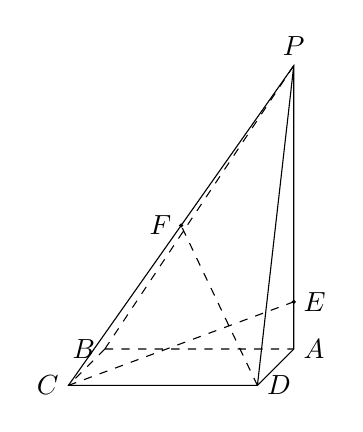
\begin{tikzpicture}[>=latex,scale = 0.6]
\draw (0,0,0) node [right] {$A$} coordinate (A);
\draw (0,6,0) node [above] {$P$} coordinate (P);
\draw (-4,0,0) node [left] {$B$} coordinate (B);
\draw (-4,0,2) node [left] {$C$} coordinate (C);
\draw (0,0,2) node [right] {$D$} coordinate (D);
\filldraw ($(C)!0.5!(P)$) circle (0.03) node [left] {$F$} coordinate (F);
\filldraw ($(A)!{1/6}!(P)$) circle (0.03) node [right] {$E$} coordinate (E);
\draw (A) -- (P) -- (C) -- (D) -- cycle (P) -- (D);
\draw [dashed] (B) -- (P) (B) -- (C) (B) -- (A) (C) -- (E) (D) -- (F);
\end{tikzpicture}
\end{center}
(1) 求三棱锥$E-ABD$的体积;\\
(2) 求异面直线$CE$与$DF$所成角的大小.
\item 设$z+1$为关于$x$的方程$x^2+mx+n=0$, $m,n\in\mathbf{R}$的虚根, $\mathrm{i}$为虚数单位.\\
(1) 当$z=-1+\mathrm{i}$时, 求$m$、$n$的值;\\
(2) 若$n=1$, 在复平面上, 设复数$z$所对应的点为$P$, 复数$2+4\mathrm{i}$所对应的点为$Q$, 试求$|PQ|$的取值范围.
\item 某渔业公司最近开发的一种新型淡水养虾技术具有方法简便且经济效益好的特点, 研究表明: 用该技术进行淡水养虾时, 在一定的条件下, 每尾虾的平均生长速度为$g(x)$(单位: 千克/年)养殖密度为$x$($x>0$, 单位: 尾/立方分米), 当$x$不超过$4$时, $g(x)$的值恒为$2$; 当$4\le x\le 20$时, $g(x)$是$x$的一次函数, 且当$x$达到$20$时, 因养殖空间受限等原因, $g(x)$的值为$0$.\\
(1) 当$0<x\le 20$时, 求函数$g(x)$的表达式;\\
(2) 在(1)的条件下, 求函数$f(x)=x\cdot g(x)$的最大值.
\item 在平面直角坐标系$xOy$中, 椭圆$\dfrac{x^2}{27}+\dfrac{y^2}{23}=1$的右焦点为双曲线$C:\dfrac{x^2}{a^2}-\dfrac{y^2}{b^2}=1$($a>0$,
$b>0$)的右顶点, 直线$x+2y+1=0$与$C$的一条渐近线平行.
\begin{center}
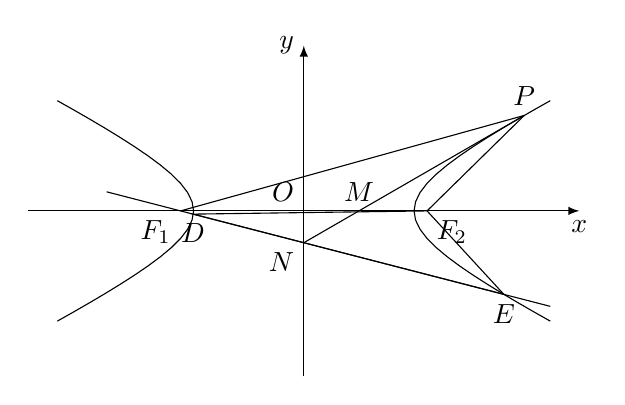
\begin{tikzpicture}[>=latex, scale = 0.7]
\draw [->] (-5,0) -- (5,0) node [below] {$x$};
\draw [->] (0,-3) -- (0,3) node [left] {$y$};
\draw (0,0) node [above left] {$O$};
\draw ({-sqrt(5)},0) node [below left] {$F_1$} coordinate (F1);
\draw ({sqrt(5)},0) node [below right] {$F_2$} coordinate (F2);
\draw (4,{sqrt(3)}) node [above] {$P$} coordinate (P);
\draw (P) -- (F1) (P) -- (F2);
\draw (1,0) node [above] {$M$} coordinate (M);
\draw ($(P)!{4/3}!(M)$) node [below left] {$N$} coordinate (N);
\draw (P) -- (N);
\draw [name path = line] ($(F1)!-0.6!(N)$) -- ($(F1)!3!(N)$);
\draw [name path = leftcurve, domain = -2:2] plot ({-sqrt(1+pow(\x,2))*2},\x);
\draw [name path = rightcurve, domain = -2:2] plot ({sqrt(1+pow(\x,2))*2},\x);
\draw [name intersections = {of = line and leftcurve, by = D}];
\draw [name intersections = {of = line and rightcurve, by = E}];
\draw (D) node [below] {$D$} -- (E) node [below] {$E$} -- (F2) -- cycle;
\end{tikzpicture}
\end{center}
(1) 求$C$的方程;\\
(2) 如图, $F_1$、$F_2$为$C$的左右焦点, 动点$P(x_0,y_0)$($y_0\ge 1$)在$C$的右支上, 且$\angle F_1PF_2$的平分线与$x$轴、$y$轴分别交于点$M(m,0)$($-\sqrt 5<m<\sqrt 5$)、$N$, 试比较$m$与$\sqrt 2$的大小, 并说明理由;\\
(3) 在(2)的条件下, 设过点$F_1$、$N$的直线$l$与$C$交于$D$、$E$两点, 求$\triangle F_2DE$的面积最大值.
\item 设$f_{(k,t)}(x)=\dfrac{kx+t}x$(这里的$k,t,x\in \mathbf{R}$且$x\ne 0$).\\
(1) $f_{(1,2)}(1)$, $f_{(2,2)}(x)$, $f_{(1,3)}(3)$成等差数列, 求$x$的值;\\
(2) 已知$\{f_{(0,1)}(\dfrac 1{x_n})\}$, $n\in \mathbf{N}^*$是公比为$\dfrac 32$的等比数列, $x_1,x_5\in \mathbf{N}^*$. 是否存在正整数$u$, 使
得$x_1\ge u^4$, 且$x_5\le (u+1)^4$? 若存在, 求出$u$的值, 若不存在, 请说明理由;\\
(3) 如果存在正常数$M$, 使得$|y_n|\le M$对一切$n\in \mathbf{N}^*$恒成立, 那么称数列有界. 已知$a>0$, $m$为正偶数, 数列$\{x_n\}$满足$x_1=b<0$, 且$x_{n+1}=f_{(b,a)}(\dfrac 1{x_n^m})(n\in \mathbf{N}^*)$, 证明: 若$ab^{m-1}+2\ge 0$, 则数列$\{x_n\}$有界.


%zmj15
\item 已知集合$A=\{1,2,4,6,8\}$, $B=\{x|x=2k, \ k\in A\}$, 则$A\cap B=$\blank{50}.
\item 已知$\dfrac{\overline z}{1-\mathrm{i}}=2+\mathrm{i}$, 则复数$z$的虚部为\blank{50}.
\item 设函数$f(x)=\sin x-\cos x$, 且$f(a)=1$, 则$\sin 2a=$\blank{50}.
\item 已知二元一次方程$\begin{cases} a_1x+b_1y+c_1, \\ a_2x+b_2y+c_2 \end{cases}$的增广矩阵是$\begin{pmatrix} 1 & -1 & 1 \\ 1 & 1 & 3\end{pmatrix}$, 则此方程组的解是\blank{50}.
\item 数列$\{a_n\}$是首项为$1$, 公差为$2$的等差数列, $S_n$是它前$n$项和, 则$\displaystyle\lim_{n\to\infty}\dfrac{S_n}{a_n^2}=$\blank{50}.
\item 已知角$A$是$\triangle ABC$的内角, 则``$\cos A=\dfrac 12$''是``$\sin A=\dfrac {\sqrt 3}2$''的\blank{50}条件(填``充分非必要''、``必要非充分''、``充要条件''、``既非充分又非必要''之一)
\item 若双曲线$x^2-\dfrac{y^2}{b^2}=1$的一个焦点到其渐近线距离为$2\sqrt{2}$, 则该双曲线焦距等于\blank{50}.
\item 一个底面半径为$2$的圆柱被与其底面所成角是$60^\circ$的平面所截, 截面是一个椭圆, 则该椭圆的焦距等于\blank{50}.
\begin{center}
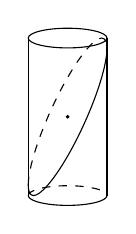
\begin{tikzpicture}[>=latex, scale = 0.5]
\draw (-1,-2) arc (180:360:1 and 0.25);
\draw (-1,2) arc (180:-180:1 and 0.25);
\draw [dashed] (-1,-2) arc (180:0:1 and 0.25);
\draw (-1,-2) -- (-1,2) (1,-2) -- (1,2);
\draw [domain = 180:360] plot ({cos(\x)},{-sqrt(3)+sin(\x)+sqrt(3)*(cos(\x)+1)});
\draw [domain = 180:0, dashed] plot ({cos(\x)},{-sqrt(3)+sin(\x)+sqrt(3)*(cos(\x)+1)});
\filldraw (0,0) circle (0.03);
\end{tikzpicture}
\end{center}
\item 设$F_1,F_2$分别是双曲线$\dfrac{x^2}{a^2}-\dfrac{y^2}{b^2}=1$($a>0$, $b>0$)的左、右焦点, 点$P$在双曲线右支上且满足$|PF_2|=|F_1F_2|$, 双曲线的渐近线方程为$4x\pm 3y=0$, 则$\cos \angle PF_1F_2=$\blank{50}.
\item 若$a,b$分别是正数$p,q$的算术平均数和几何平均数, 且$a,b,-2$这三个数可适当排序后成等差数列, 也可适当排序后成等比数列, 则$p+q+pq$的值形成的集合是\blank{50}.
\item 点$M(20,40)$, 抛物线$y^2=2px$($p>0$)的焦点为$F$, 若对于抛物线上的任意点$P$, $|PM|+|PF|$的最小值为$41$, 则$p$的值等于\blank{50}.
\item 已知数列$\{a_n\}$满足$a_1=-2$, 且$S_n=\dfrac 32a_n+n$(其中$S_n$为数列$\{a_n\}$前$n$项和), $f(x)$是定义在$\mathbf{R}$上的奇函数, 且满足$f(2-x)=f(x)$, 则$f(a_{2022})=$\blank{50}.
\item 若$a>b$, 则下列各式中恒正的是\bracket{20}.
\fourch{$\lg(a-b)$}{$a^3-b^3$}{$0.5^a-0.5^b$}{$|a|-|b|$}
\item 在空间中, $\alpha$表示平面, $m$、$n$表示两条直线, 则下列命题中错误的是\bracket{20}.
\onech{若$m\parallel \alpha$, $m$、$n$不平行, 则$n$与$\alpha$不平行}{若$m\parallel \alpha$, $m$、$n$不垂直, 则$n$与$\alpha$不垂直}{若$m\perp \alpha$, $m$、$n$不平行, 则$n$与$\alpha$不垂直}{若$m\perp \alpha$, $m$、$n$不垂直, 则$n$与$\alpha$不平行}
\item 已知函数$f(x)=A\sin(\omega x+\varphi)$($A>0$, $\omega>0$)的图像与直线$y=b$($0<b<A$)的三个相邻交点的横坐标依次是$1,2,4$, 下列区间是函数$f(x)$单调递增区间的是\bracket{20}.
\fourch{$[0,3]$}{$[\dfrac 32,3]$}{$[3,6]$}{$[3,\dfrac 92]$}
\item 已知点$M(a,b)$与点$N(0,-1)$在直线的两侧, 给出以下结论:
\textcircled{1} $3a-4b+5>0$;\\
\textcircled{2} 当$a>0$时, $a+b$有最小值, 无最大值;\\
\textcircled{3} $a^2+b^2>1$;\\
\textcircled{4} 当$a>0$且$a\ne 1$时, $\dfrac{b+1}{a-1}$的取值范围是$(-\infty,-\dfrac 94)\cup (\dfrac 34,+\infty)$;\\
正确的个数是
\fourch{$1$}{$2$}{$3$}{$4$}
\item 如图在三棱锥$P-ABC$中, 棱$AB$、$AC$、$AP$两两垂直, $AB=AC=AP=3$, 点$M$在$AP$上, 且$AM=1$.
\begin{center}
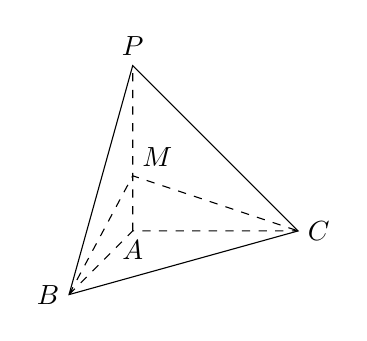
\begin{tikzpicture}[>=latex,scale = 0.7]
\draw (0,0,0) node [below] {$A$} coordinate (A);
\draw (3,0,0) node [right] {$C$} coordinate (C);
\draw (0,0,3) node [left] {$B$} coordinate (B);
\draw (0,3,0) node [above] {$P$} coordinate (P);
\draw (0,1,0) node [above right] {$M$} coordinate (M);
\draw (P) -- (B) -- (C) -- cycle;
\draw [dashed] (A) -- (P) (B) -- (A) -- (C) (B) -- (M) -- (C);
\end{tikzpicture}
\end{center}
(1) 求异面直线$BM$和$PC$所成的角的大小;\\
(2) 求三棱锥$P-BMC$的体积.
\item 已知函数$f(x)=(a+1)x^2+(a-1)x+(a^2-1)$, 其中$a\in \mathbf{R}$\\
(1) 当$f(x)$是奇函数时, 求实数$a$的值;\\
(2) 当函数$f(x)$在$[2,+\infty)$上单调递增时, 求实数$a$的取值范围.
\item 如图所示, $A$,$B$两处各有一个垃圾中转站, $B$在$A$的正东方向$16\text{km}$处, $AB$的南面为居民生活区. 为了妥善处理生活垃圾, 政府决定在$AB$的北面$P$处建一个发电厂, 利用垃圾发电. 要求发电厂到两个垃圾中转站的距离(单位: $\text{km}$)与它们每天集中的生活垃圾量(单位: 吨)成反比, 现估测得$A,B$两处中转站每天集中的生活垃圾量分别约为$30$吨和$50$吨.
\begin{center}
\begin{tikzpicture}[>=latex]
\filldraw (0,0) circle (0.05) node [left] {$A$} coordinate (A) -- (3,0) circle (0.05) node [right] {$B$} coordinate (B);
\path [name path = c1] (A) ++ (3,0) arc (0:40:3);
\path [name path = c2] (B) ++ (-1.8,0) arc (180:100:1.8);
\path [name intersections = {of = c1 and c2, by = P}];
\draw [dotted] (A) -- (P) node [above] {$P$} -- (B);
\filldraw (P) circle (0.03);
\draw [->] (3,1) -- (3,1.5) node [right] {北};
\draw (1.5,0) node [below] {居民生活区};
\end{tikzpicture}
\end{center}
(1) 当$AP=15\text{km}$时, 求$\angle APB$的值;\\
(2) 发电厂尽量远离居民区, 要求$\triangle PAB$的面积最大. 问此时发电厂与两个垃圾中转站的距离各为多少?
\item 已知点$A(-1,0)$, $B(1,0)$, 直线$l:ax+by+c=0$(其中$a,b,c\in \mathbf{R}$), 点$P$在直线$l$上.\\
(1) 若$a,b,c$是常数列, 求$|PB|$的最小值;\\
(2) 若$a,b,c$成等差数列, 且$PA\perp l$, 求$|PB|$的最大值;\\
(3) 若$a,b,c$成等比数列, 且$PA\perp l$, 求$|PB|$的取值范围.
\item 已知函数$f(x)=2-|x|$, 无穷数列满足$\{a_n\}$满足$a_{n+1}=f(a_n)$, $n\in \mathbf{N}^*$.\\
(1) 若$a_1=2$, 写出数列的通项公式(不必证明);\\
(2) 若$a_1>0$, 且$a_1,a_2,a_3$成等比数列, 求$a_1$的值; 此时$\{a_n\}$是否为等比数列, 说明理由;\\
(3) 证明: $a_1,a_2,\cdots,a_n,\cdots$成等差数列的一个充要条件是$a_1=1$.

%zmj16
\item 已知集合$A=\{1,2,3,4\}$, $B=\{3,4,5\}$, 则$A\cap B=$\blank{50}.
\item 若排列数$\mathrm{P}_6^m=6\times 5\times 4$, 则$m=$\blank{50}.
\item 不等式$\dfrac{x-1}{x}>1$的解集为\blank{50}.
\item 已知球的体积为$36\pi$, 则该球主视图的面积等于\blank{50}.
\item 已知复数$z$满足$z+\dfrac{3}{z}=0$, 则$|z|=$\blank{50}.
\item 设双曲线$\dfrac{x^2}{9}-\dfrac{y^2}{b^2}=1 \ (b>0)$的焦点为$F_1$、$F_2$, $P$为该双曲线上的一点, 若$|PF_1|=5$, 则$|PF_2|=$\blank{50}.
\item 如图, 以长方体$ABCD-A_1B_1C_1D_1$的顶点$D$为坐标原点, 过$D$的三条棱所在的直线为坐标轴, 建立空间直角坐标系. 若$\overrightarrow{DB_1}$的坐标为$(4,3,2)$, 则$\overrightarrow{AC_1}$的坐标是\blank{50}.
\begin{center}
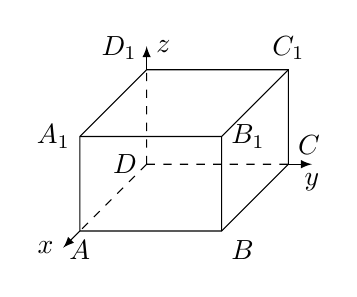
\begin{tikzpicture}[>=latex, scale = 0.6]
\draw [dashed] (0,0) node [left] {$D$} -- (3,0) node [above right] {$C$} (0,0) -- (225:2) node [below] {$A$}  (0,0) -- (0,2) node [above left] {$D_1$};
\draw (3,0) -- (3,2) node [above] {$C_1$} -- (0,2) --++ (225:2) node [left] {$A_1$} --++ (0,-2) --++ (3,0) node [below right] {$B$} -- cycle;
\draw (0,2) ++ (225:2) --++ (3,0) node [right] {$B_1$} --+ (45:2) (3,0) ++ (225:2) --+ (0,2);
\draw [->] (3,0) -- (3.5,0) node [below] {$y$};
\draw [->] (0,2) -- (0,2.5) node [right] {$z$};
\draw [->] (225:2) -- (225:2.5) node [left] {$x$};
\end{tikzpicture}
\end{center}
\item 定义在$(0,+\infty)$上的函数$y=f(x)$的反函数为$y=f^{-1}(x)$. 若$g(x)=\begin{cases}3^x-1, & x\le 0,\\ f(x), & x>0\end{cases}$为奇函数, 则$f^{-1}(x)=2$的解为\blank{50}.
\item 已知四个函数: \textcircled{1} $y=-x$, \textcircled{2} $y=-\dfrac{1}{x}$, \textcircled{3} $y=x^3$, \textcircled{4} $y=x^{\frac{1}{2}}$. 从中任选$2$个, 则事件``所选$2$个函数的图像有且仅有一个公共点''的概率为\blank{50}.
\item 已知数列$\{a_n\}$和$\{b_n\}$, 其中$a_n=n^2, \ n\in \mathbf{N}^*$, $\{b_n\}$的项是互不相等的正整数. 若对于任意$n\in \mathbf{N}^*$, $\{b_n\}$的第$a_n$项等于$\{a_n\}$的第$b_n$项, 则$\dfrac{\lg (b_1b_4b_9b_{16})}{\lg(b_1b_2b_3b_4)}=$\blank{50}.
\item 设$\alpha_1,\alpha_2\in \mathbf{R}$, 且$\dfrac{1}{2+\sin\alpha_1}+\dfrac{1}{2+\sin(2\alpha_2)}=2$, 则$|10\pi-\alpha_1-\alpha_2|$的最小值等于\blank{50}.
\item 如图, 用$35$个单位正方形拼成一个矩形, 点$P_1,P_2,P_3,P_4$以及四个标记为``
\begin{tikzpicture}
\filldraw ({-0.0625*sqrt(3)},-0.0625) -- ({0.0625*sqrt(3)},-0.0625) -- (0,0.125) -- cycle;
\end{tikzpicture}''的点在正方形的顶点处, 设集合$\Omega=\{P_1,P_2,P_3,P_4\}$, 点$P\in \Omega$. 过$P$作直线$l_P$, 使得不在$l_P$上的``
\begin{tikzpicture}
\filldraw ({-0.0625*sqrt(3)},-0.0625) -- ({0.0625*sqrt(3)},-0.0625) -- (0,0.125) -- cycle;
\end{tikzpicture}''的点分布在$l_P$的两侧. 用$D_1(l_P)$和$D_2(l_P)$分别表示$l_P$一侧和另一侧的``
\begin{tikzpicture}
\filldraw ({-0.0625*sqrt(3)},-0.0625) -- ({0.0625*sqrt(3)},-0.0625) -- (0,0.125) -- cycle;
\end{tikzpicture}''的点到$l_P$的距离之和. 若过$P$的直线$l_P$中有且只有一条满足$D_1(l_P)=D_2(l_P)$, 则$\Omega$中所有这样的$P$为\blank{50}.
\begin{center}
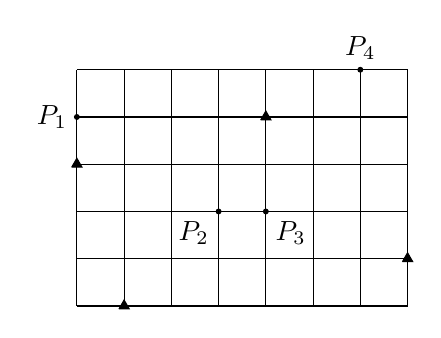
\begin{tikzpicture}[scale = 0.6]
\foreach \i in {0,1,2,3,4,5,6,7}{\draw (\i,0) -- (\i,5);};
\foreach \i in {0,1,2,3,4,5}{\draw (0,\i) -- (7,\i);};
\filldraw  (1,0) ++ ({-0.0625*sqrt(3)},-0.0625) coordinate(P) --++ ({2*0.0625*sqrt(3)},0) --++ ({-0.0625*sqrt(3)},{3*0.0625}) -- (P);
\filldraw  (7,1) ++ ({-0.0625*sqrt(3)},-0.0625) coordinate(P) --++ ({2*0.0625*sqrt(3)},0) --++ ({-0.0625*sqrt(3)},{3*0.0625}) -- (P);
\filldraw  (0,3) ++ ({-0.0625*sqrt(3)},-0.0625) coordinate(P) --++ ({2*0.0625*sqrt(3)},0) --++ ({-0.0625*sqrt(3)},{3*0.0625}) -- (P);
\filldraw  (4,4) ++ ({-0.0625*sqrt(3)},-0.0625) coordinate(P) --++ ({2*0.0625*sqrt(3)},0) --++ ({-0.0625*sqrt(3)},{3*0.0625}) -- (P);
\filldraw (0,4) circle (0.05) node [left] {$P_1$};
\filldraw (3,2) circle (0.05) node [below left] {$P_2$};
\filldraw (4,2) circle (0.05) node [below right] {$P_3$};
\filldraw (6,5) circle (0.05) node [above] {$P_4$};
\end{tikzpicture}
\end{center}
\item 关于$x$、$y$的二元一次方程组$\begin{cases}
x+5y=0, \\ 2x+3y=4\end{cases}$的系数行列式$D$为\bracket{15}.
\fourch{$\begin{vmatrix}
0 & 5 \\ 4 & 3
\end{vmatrix}$}{$\begin{vmatrix}
1 & 0 \\ 2 & 4
\end{vmatrix}$}{$\begin{vmatrix}
1 & 5 \\ 2 & 3
\end{vmatrix}$}{$\begin{vmatrix}
6 & 0 \\ 5 & 4
\end{vmatrix}$}
\item 在数列$\{a_n\}$中, $a_n=\left(-\dfrac{1}{2}\right)^n, \ n\in \mathbf{N}^*$, 则$\displaystyle\lim_{n\to \infty}a_n$\bracket{15}.
\fourch{等于$-\dfrac{1}{2}$}{等于$0$}{等于$\dfrac{1}{2}$}{不存在}
\item 已知$a,b,c$为实常数, 数列$\{x_n\}$的通项$x_n=an^2+bn+c, \ n\in \mathbf{N}^*$, 则``存在$k\in \mathbf{N}^*$, 使得$x_{100+k},x_{200+k},x_{300+k}$成等差数列''的一个必要条件是\bracket{15}.
\fourch{$a\ge 0$}{$b\le 0$}{$c=0$}{$a-2b+c=0$}
\item 在平面直角坐标系$xOy$中, 已知椭圆$C_1:\dfrac{x^2}{36}+\dfrac{y^2}{4}=1$和$C_2:x^2+\dfrac{y^2}{9}=1$. $P$为$C_1$上的动点, $Q$为$C_2$上的动点, $w$是$\overrightarrow{OP}\cdot \overrightarrow{OQ}$的最大值. 记$\Omega=\{(P,Q)|P\text{在}C_1\text{上}, \ Q\text{在}C_2\text{上, 且}\overrightarrow{OP}\cdot \overrightarrow{OQ}=w\}$, 则$\Omega$中的元素有\bracket{15}.
\fourch{$2$个}{$4$个}{$8$个}{无穷个}
\item 如图, 直三棱柱$ABC-A_1B_1C_1$的底面为直角三角形, 两直角边$AB$和$AC$的长分别为$4$和$2$, 侧棱$AA_1$的长为$5$.\\
(1) 求三棱柱$ABC-A_1B_1C_1$的体积;\\
(2) 设$M$是$BC$中点, 求直线$A_1M$与平面$ABC$所成角的大小.
\begin{center}
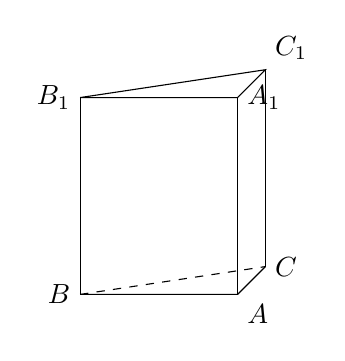
\begin{tikzpicture}[scale=0.5]
\draw (0,0) node [below right] {$A$} coordinate (A) -- (-4,0) node [left] {$B$} coordinate (B) (0,0) -- (45:1) node [right] {$C$} coordinate (C);
\draw [dashed] (B) -- (C);
\draw (A) --++ (0,5) node [right] {$A_1$} coordinate (A1) ;
\draw (B) --++ (0,5) node [left] {$B_1$} coordinate (B1);
\draw (C) --++ (0,5) node [above right] {$C_1$} coordinate (C1);
\draw (A1) -- (B1) -- (C1) -- cycle;				
\end{tikzpicture}
\end{center}
\item 已知函数$f(x)=\cos^2 x-\sin^2 x+\dfrac{1}{2}, \ x\in (0,\pi)$.\\
(1) 求$f(x)$的单调递增区间;\\
(2) 设$\triangle ABC$为锐角三角形, 角$A$所对的边$a=\sqrt{19}$, 角$B$所对的边$b=5$, 若$f(A)=0$, 求$\triangle ABC$的面积.
\item 根据预测, 某地第$n \ (n\in \mathbf{N}^*)$个月共享单车的投放量和损失量分别为$a_n$和$b_n$(单位: 辆), 其中$a_n=\begin{cases}
5n^4+15, & 1\le n\le 3,\\ -10n+470, & n \ge 4,
\end{cases}$ $b_n=n+5$, 第$n$个月底的共享单车的保有量是前$n$个月的累计投放量与累计损失量的差.\\
(1) 求该地区第$4$个月底的共享单车的保有量;\\
(2) 已知该地共享单车停放点第$n$个月底的单车容纳量$S_n=-4(n-46)^2+8800$(单位: 辆). 设在某月底, 共享单车保有量达到最大, 问该保有量是否超出了此时停放点的单车容纳量?
\item 在平面直角坐标系$xOy$中, 已知椭圆$\Gamma: \dfrac{x^2}{4}+y^2=1$, $A$为$\Gamma$的上顶点, $P$为$\Gamma$上异于上、下顶点的动点. $M$为$x$正半轴上的动点.\\
(1) 若$P$在第一象限, 且$|OP|=\sqrt{2}$, 求$P$的坐标;\\
(2) 设$P\left(\dfrac{8}{5},\dfrac{3}{5}\right)$. 若以$A,P,M$为顶点的三角形是直角三角形, 求$M$的横坐标;\\
(3) 若$|MA|=|MP|$, 直线$AQ$与$\Gamma$交于另一点$C$, 且$\overrightarrow{AQ}=2\overrightarrow{AC}$, $\overrightarrow{PQ}=4\overrightarrow{PM}$, 求直线$AQ$的方程.
\item 设定义在$\mathbf{R}$上的函数$f(x)$满足: 对于任意的$x_1,x_2\in \mathbf{R}$, 当$x_1<x_2$时, 都有$f(x_1)\le f(x_2)$.\\
(1) 若$f(x)=ax^3+1$, 求$a$的取值范围;\\
(2) 若$f(x)$是周期函数, 证明: $f(x)$是常值函数;\\
(3) 设$f(x)$恒大于零. $g(x)$是定义在$\mathbf{R}$上的、恒大于零的周期函数, $M$是$g(x)$的最大值. 函数$h(x)=f(x)g(x)$. 证明: ``$h(x)$是周期函数''的充要条件是``$f(x)$是常值函数''.

\end{enumerate}


\iffalse













\fi

































\end{document}